\PassOptionsToPackage{quiet}{fontspec}
\documentclass[12pt,a4paper]{article}
\usepackage{thesis} % 格式控制
\usepackage{indentfirst}
\usepackage{enumitem}
\usepackage{amsmath} % 数学公式支持
\usepackage{amsfonts} % 数学字体支持
\usepackage{amssymb} % 数学符号支持
\usepackage{graphicx} % 图片插入支持
\usepackage{float} % 浮动体位置控制，支持 [H] 选项
\usepackage{caption} % 图表标题格式控制
\usepackage{geometry} % 页面布局控制
\usepackage{setspace} % 行距控制
\usepackage{xeCJK} % 中文字体支持
\usepackage{fontspec} % 字体设置
\usepackage[most]{tcolorbox} % 高亮按键命令
\usepackage{listings} % 代码高亮
\usepackage{xcolor} % 颜色支持
\setlength{\parindent}{2em} % 控制首行缩进  
\addtolength{\parskip}{3pt} % 控制段落距离  
\onehalfspacing % 1.5倍行距  
\graphicspath{{./figures/}} % 指定图片所在文件夹  
\setCJKmainfont{SimSun}

% 配置lstlisting样式
\lstset{
    basicstyle=\ttfamily\small,
    breaklines=true,
    frame=single,
    numbers=left,
    numberstyle=\tiny\color{gray},
    backgroundcolor=\color{gray!10},
    keywordstyle=\color{blue},
    commentstyle=\color{green!60!black},
    stringstyle=\color{red},
    showstringspaces=false,
    tabsize=4,
    captionpos=b,
    xleftmargin=2em,
    xrightmargin=2em,
    aboveskip=1em,
    belowskip=1em
}

\classname{\heiti\bfseries 计算机组成与设计}  % 设置课程名称
\makepagestyle{}{}

\newtcbox{\keyblue}{on line,
  colframe=blue!60!black, colback=blue!5,
  boxrule=0.8pt, arc=2pt, boxsep=0pt, left=3pt, right=3pt, top=2pt, bottom=2pt,
  tcbox raise base, fontupper=\ttfamily\small}

\newtcbox{\pathbox}{on line,
  colframe=green!60!black, colback=green!5,
  boxrule=0.8pt, arc=2pt, boxsep=0pt, left=3pt, right=3pt, top=2pt, bottom=2pt,
  tcbox raise base, fontupper=\ttfamily\small}

\begin{document}
\maketitlepage{浮点加操作指令及硬件扩展设计}{玉泉教7-104}{郑智瑄}{3230103913}{\today}{赵武锋} %封面页 

\maketoc

\section{实验概述}

\subsection{Project1简介}
本次project基于著名的开源SoC（System on Chips）项目VeeRwolf，VeeRwolf所采用的RISC-V核心是EL2，也是著名的开源项目。

EL2是一个四级流水线的简单但完整的RISC-V处理器，支持RV32IMC指令集，但是不原生支持浮点操作。本project需要按照指示，完成EL2的指令集及硬件集成，使之支持单精度的基于IEEE 754标准的浮点加操作。



\subsection{实验环境}
\begin{itemize}[itemsep=0pt, parsep=3pt]
    \item \textbf{操作系统}：Windows 11 + WSL2 (Ubuntu22.04)
    \item \textbf{开发工具}：VS Code + WSL扩展
    \item \textbf{仿真器}：Verilator
    \item \textbf{波形查看器}：GTKWave
    \item \textbf{编译平台}：Catapult-studio (可选)
    \item \textbf{硬件描述语言}：SystemVerilog
\end{itemize}

\section{环境搭建}

\subsection{WSL2安装与配置}

WSL2 (Windows Subsystem for Linux 2) 是Windows 10/11支持的轻量级Linux虚拟机，非常适合中小型体量的Linux工程搭建和运行。

\subsubsection{安装步骤}
\begin{enumerate}[itemsep=0pt, parsep=3pt]
    \item 以管理员身份打开PowerShell
    \item 执行命令 \keyblue{wsl --install}，启用WSL及虚拟机功能，下载WSL2内核并安装Ubuntu发行版
    \item 根据提示设置Ubuntu用户名和密码
    \item 执行 \keyblue{wsl --list} 验证安装成功
    \item 执行 \keyblue{wsl} 或 \keyblue{bash} 进入Ubuntu系统
    \item 执行 \keyblue{sudo apt update} 更新软件包列表
    \item 执行 \keyblue{sudo apt install -y build-essential} 安装基本开发工具
\end{enumerate}

\subsection{VS Code配置}

\begin{enumerate}[itemsep=0pt, parsep=3pt]
    \item 在VS Code中安装WSL扩展和Remote Explorer扩展
    \item 通过Remote Explorer连接到Ubuntu虚拟机
    \item 将工程文件夹挂载到WSL环境中
\end{enumerate}

挂载路径转换规则：将Windows路径中的 \texttt{\textbackslash} 替换为 \texttt{/}，将盘符 \texttt{C:} 替换为 \texttt{/mnt/c}。

例如:Windows路径：\pathbox{C:\textbackslash Users\textbackslash xxx\textbackslash RVfpga\_NexysA7-DDR}

转换为WSL路径：\pathbox{/mnt/c/Users/xxx/RVfpga\_NexysA7-DDR}

\subsection{工具链安装}

\subsubsection{Verilator仿真器}
\begin{lstlisting}[language=bash]
sudo apt-get install git make autoconf g++ flex bison libfl2 libfl-dev
sudo apt-get install verilator
verilator --version  # 验证安装
\end{lstlisting}

\subsubsection{GTKWave波形查看器}
\begin{lstlisting}[language=bash]
sudo apt-get install gtkwave
gtkwave  # 验证安装
\end{lstlisting}

\subsubsection{Catapult-studio编译平台（可选）}
\begin{lstlisting}[language=bash]
mv /mnt/c/path/to/catapult-sdk_1.9.1.deb /home/username/
cd ~
sudo apt install ./catapult-sdk*.deb
cd ~/catapult-sdk_examples/1.9.1
source ./set_sdk_path.sh
catapult-studio  # 验证安装
\end{lstlisting}

\section{硬件设计与实现}

\subsection{译码级信号修改}

为了支持浮点加指令，需要在译码级添加相应的控制信号 \texttt{fp\_p}。

\subsubsection{el2\_dec\_decode\_ctl.sv修改}

在输出信号中添加 \texttt{fp\_p} 信号：
\begin{lstlisting}[language=Verilog]
output logic fp_p,
\end{lstlisting}

\subsubsection{el2\_dec.sv修改}

在输出信号中添加 \texttt{fp\_p} 信号：
\begin{lstlisting}[language=Verilog]
output logic fp_p,
\end{lstlisting}

\subsubsection{el2\_exu.sv修改}

在输入信号中添加 \texttt{fp\_p} 信号，并在除法器例化时连接该信号：
\begin{lstlisting}[language=Verilog]
input logic fp_p,

el2_exu_div_ctl divider(
    ...
    .fp(fp_p),
    ...
);
\end{lstlisting}

\subsubsection{el2\_veer.sv修改}

在连接信号中添加 \texttt{fp\_p} 信号，确保信号从顶层模块正确传递。

\subsection{浮点加法器集成}

\subsubsection{el2\_exu\_div\_ctl.sv修改}

将浮点加法器模块 \texttt{fp\_adder} 集成到整数除法器模块 \texttt{el2\_exu\_div\_ctl} 中，复用除法器的控制信号和数据通路。使用提供的修改模块 \texttt{el2\_exu\_div\_ctl\_2.sv}。

\textbf{关键设计要点：}

\begin{enumerate}[itemsep=0pt, parsep=3pt]
    \item \textbf{操作数锁存}：由于 \texttt{dividend} 和 \texttt{divisor} 信号只持续1-2个时钟周期，而浮点加法器需要多个周期读取操作数，因此需要添加寄存器链进行锁存
    \item \textbf{握手信号生成}：通过寄存器链延拓 \texttt{stb} 信号，生成 \texttt{stb\_for\_fp}，确保浮点加法器能够正确捕获操作数
    \item \textbf{操作类型识别}：设计 \texttt{fp\_operation\_latch} 模块，根据 \texttt{dp.valid}、\texttt{fp.fp\_add} 等信号识别当前操作类型
    \item \textbf{完成信号复用}：使用 \texttt{active\_operation} 信号选择浮点加法器的 \texttt{fpadd\_done} 或整数除法器的 \texttt{finish\_dly}
    \item \textbf{结果输出复用}：根据操作类型，选择输出浮点加法结果 \texttt{out\_fpadd} 或整数除法结果 \texttt{out\_raw}
\end{enumerate}

\textbf{主要修改内容：}

\paragraph{1. 信号定义}

首先定义浮点加法器所需的信号和寄存器链：

\begin{lstlisting}[language=Verilog]
wire [31:0] out_fpadd;           // 浮点加法输出结果
wire fpadd_done;                 // 浮点加法完成信号
wire stb;                        // 握手信号（strobing signal）
reg  stb_d, stb_dd;              // 握手信号的1级和2级延时
wire stb_for_fp;                 // 延拓后的握手信号
reg [31:0] divisor_d, divisor_dd;    // divisor的1级和2级寄存器
reg [31:0] dividend_d;               // dividend的1级寄存器
wire [31:0] dividend_for_fp;     // 延拓后的操作数A
wire [31:0] divisor_for_fp;      // 延拓后的操作数B
\end{lstlisting}

\textbf{说明}：这些信号用于解决操作数持续时间短的问题。原始的 \texttt{dividend} 和 \texttt{divisor} 信号只在1-2个时钟周期内有效，而浮点加法器的状态机需要多个周期来读取操作数。

\paragraph{2. 操作数锁存}

使用寄存器链锁存操作数和握手信号：

\begin{lstlisting}[language=Verilog]
// 生成握手信号
assign stb = fp.fp_add;

// 在时钟上升沿锁存信号
always @(posedge clk) begin
    stb_d <= stb;              // 握手信号延时1个时钟周期
    stb_dd <= stb_d;           // 握手信号延时2个时钟周期
    divisor_d <= divisor;      // divisor延时1个时钟周期
    divisor_dd <= divisor_d;   // divisor延时2个时钟周期
    dividend_d <= dividend;    // dividend延时1个时钟周期
end
\end{lstlisting}

\textbf{说明}：通过寄存器链保存历史数据，形成3个时钟周期的数据窗口。\texttt{stb} 信号在浮点加法操作有效时拉高。

\paragraph{3. 信号延拓}

使用或运算延长信号的有效时间：

\begin{lstlisting}[language=Verilog]
// 将3个时钟周期的信号通过或运算合并
assign stb_for_fp = stb | stb_d | stb_dd;
assign divisor_for_fp = divisor | divisor_d | divisor_dd;
assign dividend_for_fp = dividend | dividend_d;
\end{lstlisting}

\textbf{说明}：或运算确保只要历史窗口中任何一个周期有数据，延拓后的信号就保持有效。这样 \texttt{stb\_for\_fp} 可以维持3个时钟周期，给浮点加法器充足的时间读取操作数。

\paragraph{4. 浮点加法器例化}

实例化 \texttt{fp\_adder} 模块并连接信号：

\begin{lstlisting}[language=Verilog]
fp_adder simple_fp_adder(
    .input_a(dividend),          // 操作数A：直接使用dividend
    .input_b(divisor_for_fp),    // 操作数B：使用延拓后的divisor
    .input_a_stb(stb_for_fp),    // A的握手信号：延拓后的stb
    .input_b_stb(stb_for_fp),    // B的握手信号：延拓后的stb
    .output_z_ack(1),            // 输出应答：始终准备接收（tied to 1）
    .clk(clk),                   // 时钟信号
    .rst(~rst_l),                // 复位信号：低电平有效转高电平有效
    .output_z(out_fpadd),        // 输出：浮点加法结果
    .output_z_stb(fpadd_done),   // 输出有效信号：表示计算完成
    .input_a_ack(),              // A的应答信号：悬空（未使用）
    .input_b_ack()               // B的应答信号：悬空（未使用）
);
\end{lstlisting}

\textbf{说明}：\texttt{fp\_adder} 使用握手协议，\texttt{\_stb} 信号表示数据有效，\texttt{\_ack} 信号表示准备好接收。\texttt{output\_z\_ack} 设为1表示始终准备接收结果。

\paragraph{5. 操作类型识别}

实例化操作类型锁存模块：

\begin{lstlisting}[language=Verilog]
wire [3:0] active_operation;
fp_operation_latch op_latch(
    .clk(clk),
    .dp_valid(dp.valid),         // 除法有效信号
    .fp_add(fp.fp_add),          // 浮点加法使能
    .fp_mul(fp.fp_mul),          // 浮点乘法使能（预留扩展）
    .fp_div(fp.fp_div),          // 浮点除法使能（预留扩展）
    .a(active_operation)         // 输出独热码：[3]整除 [2]浮加 [1]浮乘 [0]浮除
);
\end{lstlisting}

\textbf{说明}：\texttt{fp\_operation\_latch} 模块根据输入的使能信号，输出独热码表示当前活跃的操作类型。这个模块会锁存操作类型，直到操作完成。

\paragraph{6. 完成信号多路选择}

根据操作类型选择相应的完成信号：

\begin{lstlisting}[language=Verilog]
assign finish_dly_div_fp = 
    ({32{active_operation[3]}} & {32{finish_dly}}) |     // 整数除法完成
    ({32{active_operation[2]}} & {32{fpadd_done}});      // 浮点加法完成
\end{lstlisting}

\textbf{说明}：使用位复制（\texttt{\{32\{bit\}\}}）将单个控制位扩展为32位掩码，然后通过与运算和或运算实现多路选择。当 \texttt{active\_operation[3]=1} 时选择 \texttt{finish\_dly}，当 \texttt{active\_operation[2]=1} 时选择 \texttt{fpadd\_done}。

\paragraph{7. 结果输出多路选择}

根据操作类型选择相应的输出结果：

\begin{lstlisting}[language=Verilog]
assign out[31:0] = 
    ({32{active_operation[3]}} & {32{finish_dly}} & out_raw[31:0]) |    // 整数除法结果
    ({32{active_operation[2]}} & {32{fpadd_done}} & out_fpadd[31:0]);   // 浮点加法结果
\end{lstlisting}

\textbf{说明}：采用双重掩码机制：第一层掩码根据操作类型选择通路，第二层掩码确保只有在完成信号有效时才输出结果。这种设计避免了输出中间状态的错误数据。

\textbf{设计说明：}

\begin{itemize}[itemsep=0pt, parsep=3pt]
    \item \textbf{寄存器链设计}：通过3级寄存器链（\texttt{stb}、\texttt{stb\_d}、\texttt{stb\_dd}）延长握手信号有效时间，确保浮点加法器的状态机能够稳定读取操作数
    \item \textbf{或逻辑延拓}：使用或运算将多个时钟周期的操作数合并，保证操作数在浮点加法器读取期间始终有效
    \item \textbf{操作类型编码}：\texttt{active\_operation[3:0]} 采用独热码，\texttt{[3]}表示整数除法，\texttt{[2]}表示浮点加法，\texttt{[1][0]}预留给浮点乘除
    \item \textbf{信号复用}：通过位掩码（bit mask）实现完成信号和输出结果的多路选择，避免使用额外的MUX
\end{itemize}

\clearpage
\section{仿真验证}

\subsection{测试文件}

测试文件 \texttt{fp\_add.S} 是一个RISC-V汇编程序，用于测试浮点加法器和整数除法器的功能。主要内容如下：

\begin{lstlisting}[language={[x86masm]Assembler}]
#define INSERT_NOPS_1      nop;
#define INSERT_NOPS_2      nop; INSERT_NOPS_1
#define INSERT_NOPS_3      nop; INSERT_NOPS_2
#define INSERT_NOPS_4      nop; INSERT_NOPS_3
#define INSERT_NOPS_5      nop; INSERT_NOPS_4
#define INSERT_NOPS_6      nop; INSERT_NOPS_5
#define INSERT_NOPS_7      nop; INSERT_NOPS_6
#define INSERT_NOPS_8      nop; INSERT_NOPS_7
#define INSERT_NOPS_9      nop; INSERT_NOPS_8
#define INSERT_NOPS_10     nop; INSERT_NOPS_9

.globl main 
main:
li t3, 0x40800000       # Load float 4.0 into t3
li t4, 0x40000000       # Load float 2.0 into t4
li a3, 20               # Load integer 20 into a3 (dividend)
li a4, 4                # Load integer 4 into a4 (divisor)
REPEAT: 
INSERT_NOPS_4           # Insert 4 NOPs for pipeline spacing
.word 0x01ce8f53        # fadd.s f30, t4, t3 (2.0 + 4.0 = 6.0)
INSERT_NOPS_4           # Insert 4 NOPs for pipeline spacing
div a5, a3, a4          # Test integer division: a5 = 20 / 4 = 5
INSERT_NOPS_10          # Insert 10 NOPs for pipeline spacing
beq zero, zero, REPEAT  # Infinite loop to repeat the test
\end{lstlisting}

代码说明：
\begin{itemize}[itemsep=0pt, parsep=3pt]
    \item \textbf{NOP宏定义}：用于在流水线中插入空指令，确保非流水线模块有足够时间完成操作
    \item \textbf{浮点数加载}：\texttt{0x40800000}表示4.0，\texttt{0x40000000}表示2.0（IEEE 754格式）
    \item \textbf{fadd.s指令}：自定义的浮点加指令，编码为\texttt{0x01CE8F53}，计算$2.0 + 4.0 = 6.0$
    \item \textbf{div指令}：标准整数除法指令，验证原除法器功能未受影响
    \item \textbf{循环执行}：通过无条件跳转实现重复测试
\end{itemize}

\subsection{仿真步骤}

\subsubsection{生成仿真文件}
\begin{lstlisting}[language=bash]
cd Simulators/verilatorSIM_Trace
make
./obj_dir/Vrvfpgasim
\end{lstlisting}

编译成功表示修改的代码没有语法错误。

\subsubsection{运行仿真}
\begin{lstlisting}[language=bash]
cd RVfpga_NexysA7-DDR/Labs/Lab18/commandLine
../../../Simulators/verilatorSIM_Trace/Vrvfpgasim \
    +ram_init_file=fp_add.vh +vcd=1
# 等待3秒后按 Ctrl+C 终止
\end{lstlisting}

此步骤生成波形文件 \texttt{trace.vcd}。

\subsubsection{查看波形}
\begin{lstlisting}[language=bash]
gtkwave trace.vcd
# 在GTKWave中通过 File -> Read TCL Script File 
# 读取 test.tcl 显示预设信号
\end{lstlisting}

\subsubsection{简化仿真流程（可选）}

为了简化仿真操作，我在 \pathbox{Labs/Lab18/commandLine/Makefile} 中添加了自定义的Make目标：

\begin{lstlisting}[language=make]
vcd:
	../../../Simulators/verilatorSIM_Trace/Vrvfpgasim \
	+ram_init_file=fp_add.vh +vcd=1

gtk:
	gtkwave trace.vcd
\end{lstlisting}

添加后，可以使用更简洁的命令进行仿真：

\begin{lstlisting}[language=bash]
# 进入测试目录
cd RVfpga_NexysA7-DDR/Labs/Lab18/commandLine

# 运行仿真并生成波形文件
make vcd
# 等待3秒后按 Ctrl+C 终止

# 打开GTKWave查看波形
make gtk
\end{lstlisting}

\subsection{验证结果}

通过GTKWave查看仿真生成的波形文件，可以直观地观察到浮点加法器和整数除法器的工作状态。本节通过三张波形图展示验证过程：图\ref{fig:waveform_overview}展示完整的指令执行流程，图\ref{fig:waveform_fpadd}和图\ref{fig:waveform_div}分别展示浮点加法和整数除法的细节波形。

\subsubsection{完整波形分析}

\begin{figure}[H]
    \centering
    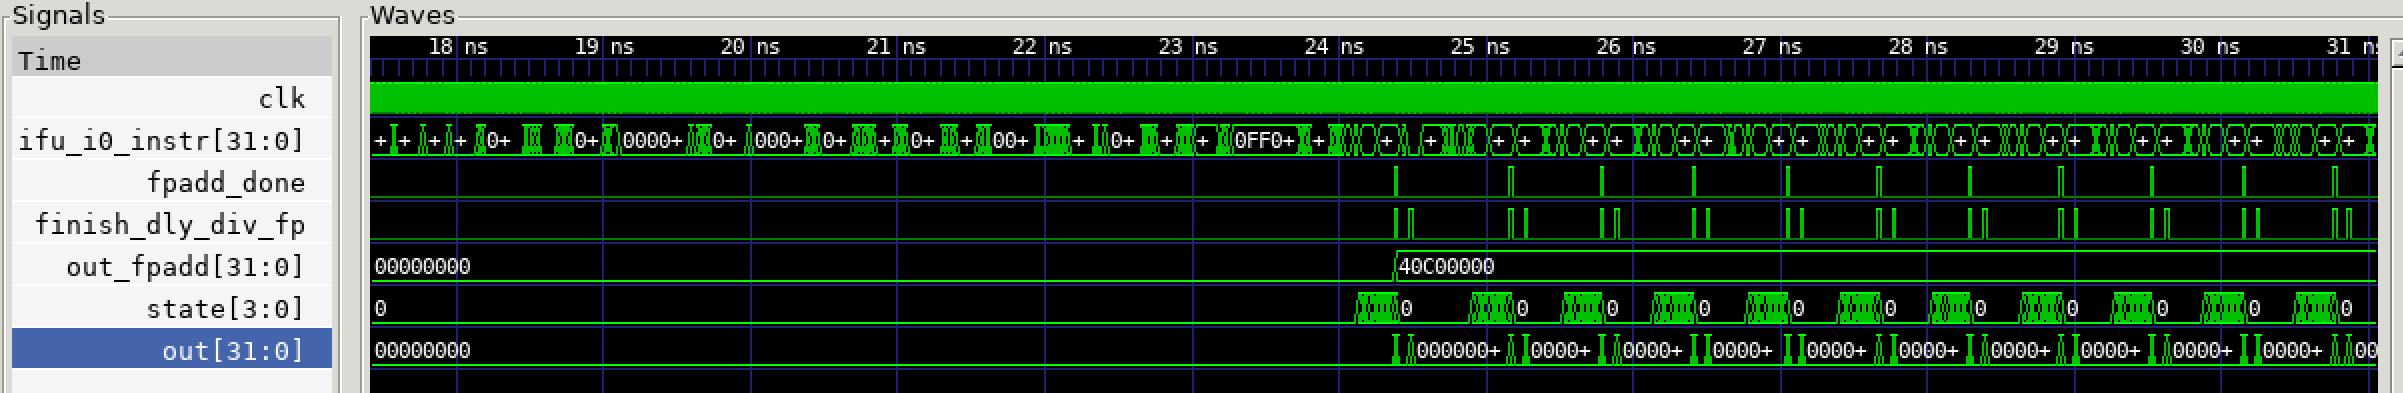
\includegraphics[width=1.0\textwidth]{p1.png}
    \caption{完整指令执行流程波形图}
    \label{fig:waveform_overview}
\end{figure}

图\ref{fig:waveform_overview}展示了从18ns到31 ns时间段内的完整仿真波形，包含了浮点加法指令和整数除法指令的连续执行。

\subsubsection{浮点加法细节波形}

\begin{figure}[H]
    \centering
    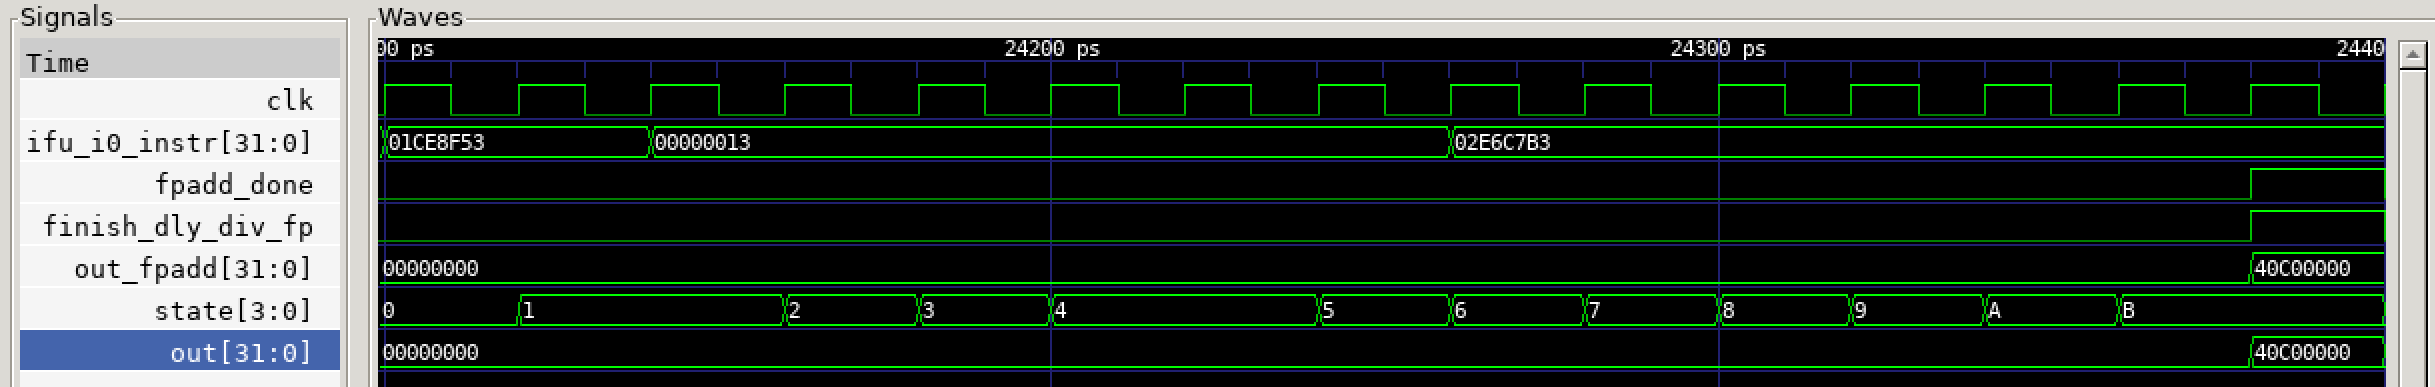
\includegraphics[width=1.0\textwidth]{p2.png}
    \caption{浮点加法运算细节波形（24.1 ns - 24.4 ns）}
    \label{fig:waveform_fpadd}
\end{figure}

图\ref{fig:waveform_fpadd}放大显示了浮点加法运算完成阶段的细节波形。

\textbf{测试参数：}
\begin{itemize}[itemsep=0pt, parsep=3pt]
    \item \textbf{指令编码}：\texttt{0x01CE8F53}（fadd.s f30, t4, t3）
    \item \textbf{操作数A}：\texttt{0x40800000}（IEEE 754格式，十进制4.0）
    \item \textbf{操作数B}：\texttt{0x40000000}（IEEE 754格式，十进制2.0）
    \item \textbf{预期结果}：\texttt{0x40C00000}（IEEE 754格式，十进制6.0）
\end{itemize}

\textbf{波形细节分析：}
\begin{itemize}[itemsep=0pt, parsep=3pt]
    \item \textbf{状态转换}：状态机从状态6→7→8→9→A→B→0，完成最后阶段的规格化和舍入操作
    \item \textbf{输出结果}：\texttt{out\_fpadd[31:0] = 0x40C00000} ✓
    \item \textbf{完成信号}：\texttt{fpadd\_done}在状态机回到0时拉高，表示计算完成
    \item \textbf{输出稳定}：\texttt{out[31:0]}信号稳定输出\texttt{0x40C00000}，随后在整数除法指令到来时变回\texttt{0x00000000}
\end{itemize}

\textbf{结果验证：}
$$4.0 + 2.0 = 6.0$$
根据IEEE 754标准：
\begin{itemize}[itemsep=0pt, parsep=3pt]
    \item \texttt{0x40800000} = $(-1)^0 \times 2^{129-127} \times 1.0 = 4.0$
    \item \texttt{0x40000000} = $(-1)^0 \times 2^{128-127} \times 1.0 = 2.0$
    \item \texttt{0x40C00000} = $(-1)^0 \times 2^{129-127} \times 1.5 = 6.0$
\end{itemize}
计算结果完全正确！

\subsubsection{整数除法细节波形}

\begin{figure}[H]
    \centering
    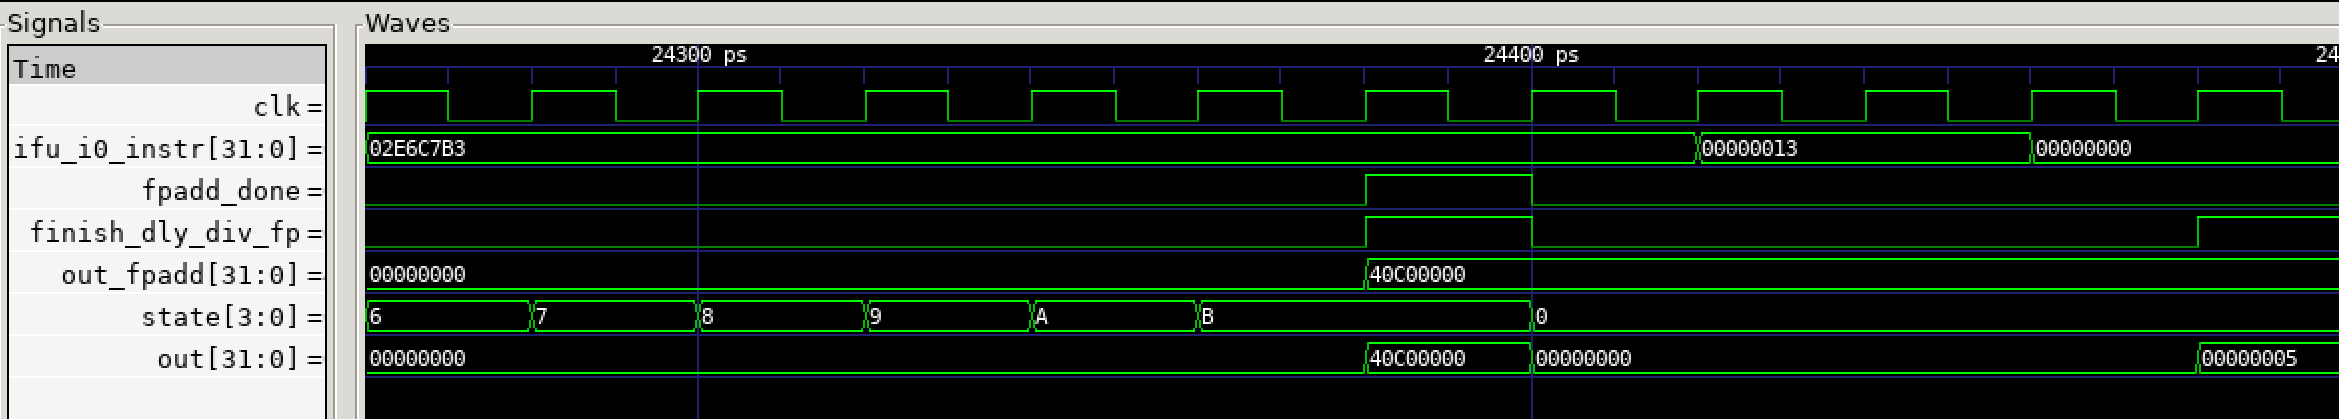
\includegraphics[width=1.0\textwidth]{p3.png}
    \caption{整数除法运算细节波形（24.3 ns - 24.5 ns）}
    \label{fig:waveform_div}
\end{figure}

图\ref{fig:waveform_div}展示了整数除法指令执行期间的细节波形，包含了高频信号的完整状态变化。

\textbf{测试参数：}
\begin{itemize}[itemsep=0pt, parsep=3pt]
    \item \textbf{指令编码}：\texttt{0x02E6C7B3}（div a5, a3, a4）
    \item \textbf{被除数}：\texttt{0x00000014}（十进制20）
    \item \textbf{除数}：\texttt{0x00000004}（十进制4）
    \item \textbf{预期结果}：\texttt{0x00000005}（十进制5）
\end{itemize}

\textbf{波形细节分析：}
\begin{itemize}[itemsep=0pt, parsep=3pt]
    \item \textbf{指令识别}：在约24 ns时刻，\texttt{ifu\_i0\_instr}显示\texttt{0x02E6C7B3}（div指令）
    \item \textbf{高频活动}：波形显示了除法器内部的迭代计算过程，\texttt{ifu\_i0\_instr}在后续周期出现高频变化
    \item \textbf{完成信号}：\texttt{finish\_dly\_div\_fp}信号多次拉高，表示除法器完成多次迭代计算
    \item \textbf{输出结果}：\texttt{out[31:0]}在除法完成后显示\texttt{0x00000005}（十进制5）✓
    \item \textbf{状态保持}：浮点加法器\texttt{state}保持在0状态，\texttt{out\_fpadd}显示\texttt{0x40C00000}（保持上次结果）
\end{itemize}

\textbf{结果验证：}
$$20 \div 4 = 5$$
整数除法运算结果正确，且原除法器功能未受浮点加法器集成的影响。

\subsubsection{信号复用机制验证}

从三张波形图的对比分析可以看出信号复用机制的正确性：

\begin{itemize}[itemsep=0pt, parsep=3pt]
    \item \textbf{浮点加法阶段}（图\ref{fig:waveform_fpadd}）：
    \begin{itemize}
        \item \texttt{out[31:0]}输出浮点加法结果\texttt{0x40C00000}
        \item \texttt{finish\_dly\_div\_fp}由\texttt{fpadd\_done}信号控制
    \end{itemize}
    
    \item \textbf{整数除法阶段}（图\ref{fig:waveform_div}）：
    \begin{itemize}
        \item \texttt{out[31:0]}切换输出整数除法结果\texttt{0x00000005}
        \item \texttt{finish\_dly\_div\_fp}由除法器的\texttt{finish\_dly}信号控制
    \end{itemize}
    
\end{itemize}

\subsubsection{验证结论}

基于以上三个层次的波形分析，得出以下验证结论：

\begin{enumerate}[itemsep=0pt, parsep=3pt]
    \item \textbf{浮点加法器功能正确}：成功实现IEEE 754标准的单精度浮点加法运算，对阶、尾数相加、规格化、舍入等步骤均正确执行
    
    \item \textbf{状态机运行稳定}：浮点加法器状态机完整经历12个状态（0→1→...→B→0），状态转换逻辑正确，无死锁或错误跳转
    
    \item \textbf{完成信号可靠}：\texttt{fpadd\_done}和\texttt{finish\_dly\_div\_fp}信号时序正确，保证了流水线的正确控制
    
    \item \textbf{原有功能完整}：整数除法器功能未受影响，迭代计算过程正常，结果准确
    
    \item \textbf{信号复用成功}：\texttt{out}信号和\texttt{finish\_dly\_div\_fp}信号的多路选择机制工作正常，能够根据操作类型正确切换输出
    
    \item \textbf{性能符合预期}：浮点加法耗时约10余个时钟周期，符合非流水线设计的性能特征
\end{enumerate}

\textbf{综合验证结果表明}：浮点加法器已成功集成到EL2处理器中，硬件功能正确，信号时序准确，完全实现了预期的设计目标。

\clearpage
\section{实验探究}

\subsection{OR运算数据保持方案的缺陷}

\subsubsection{问题提出}

在将浮点加法器集成到 \texttt{el2\_exu\_div\_ctl.sv} 时，我们采用了与整数除法器共享输入端口的设计。为了解决浮点加法器握手协议延迟导致的数据对齐问题，最初采用了\textbf{延迟链 + OR运算}的数据保持方案：

\begin{lstlisting}[language=Verilog]
// 延迟链：保存历史数据
reg [31:0] divisor_d, divisor_dd;
reg [31:0] dividend_d;

always@(posedge clk) begin
    divisor_d  <= divisor;
    divisor_dd <= divisor_d;
    dividend_d <= dividend;
end

// OR运算：尝试保持有效数据
assign divisor_for_fp  = divisor | divisor_d | divisor_dd;
assign dividend_for_fp = dividend | dividend_d;
\end{lstlisting}

\textbf{设计初衷}：
\begin{itemize}[itemsep=0pt, parsep=3pt]
    \item \texttt{dividend} 和 \texttt{divisor} 是组合逻辑信号，每个周期都可能变化
    \item fp\_adder 使用握手协议，需要2-3个时钟周期才能锁存数据
    \item 使用延迟链保存多个周期的历史值，通过OR运算确保数据保持
\end{itemize}

\textbf{理论上的问题}：当新指令到达时，如果新旧数据都非零，OR运算会导致\textbf{数据污染}：

\begin{lstlisting}[language=Verilog]
// 例如：浮点数 4.0 后紧跟整数 4
0x40800000  (浮点数 4.0，历史数据)
|
0x00000004  (整数 4，新数据)
==========
0x40800004  (错误的混合结果！)
\end{lstlisting}

这种混合值既不是有效的浮点数，也不是正确的整数，可能导致计算结果错误。

\subsubsection{验证策略}

为了验证OR运算方案是否会导致数据污染，我们设计了\textbf{零延迟背靠背测试}：

测试程序 \texttt{fp\_conflict.S}：
\begin{lstlisting}[language={[x86masm]Assembler}]
main:
    li t3, 0x40800000   # x28/f28 = 4.0
    li t4, 0x40000000   # x29/f29 = 2.0
    li a3, 20           # 被除数
    li a4, 4            # 除数

CRITICAL_TEST:
    INSERT_NOPS_4
    .word 0x01ce8f53    # fadd.s f30, f29, f28 (4.0+2.0=6.0)
    div a5, a3, a4      # 20/4=5 (紧随其后，零延迟)
    INSERT_NOPS_20
\end{lstlisting}

\textbf{测试设计要点}：
\begin{itemize}[itemsep=0pt, parsep=3pt]
    \item 使用 x28-x30 初始化数据（利用与 f28-f30 共享物理寄存器的特性）
    \item \texttt{fadd.s} 和 \texttt{div} 连续执行，无任何延迟
    \item 浮点加法需要10+周期，除法指令会在浮点运算期间到达
    \item \textbf{关键冲突点}：
    \begin{itemize}[itemsep=0pt, parsep=3pt]
        \item 浮点加法使用 \texttt{divisor = 0x40800000}（4.0）和 \texttt{divisor = 0x40000000}（2.0）
        \item 整数除法使用 \texttt{divisor = 0x00000004}（4）
        \item 如果OR运算存在问题，会产生 \texttt{0x40800000 | 0x00000004 = 0x40800004}
    \end{itemize}
\end{itemize}

\subsubsection{波形分析}

\begin{figure}[H]
    \centering
    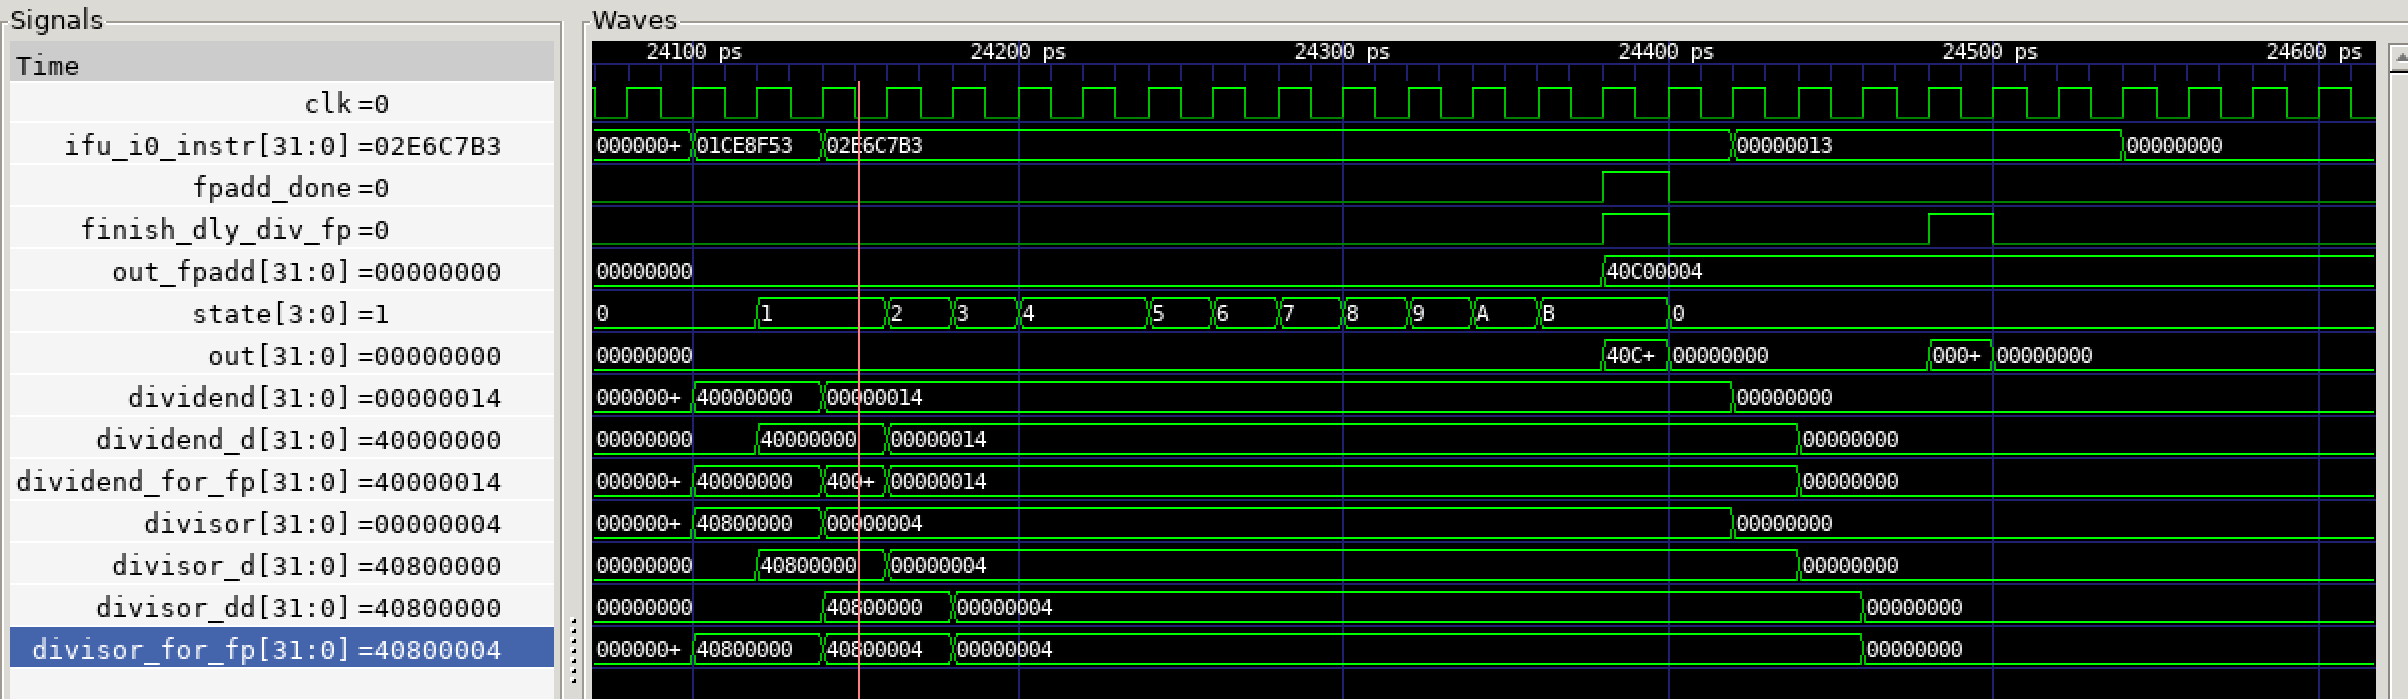
\includegraphics[width=1.0\textwidth]{ppp1.png}
    \caption{OR运算数据污染现象1}
    \label{fig:or_pollution_state}
\end{figure}

\begin{figure}[H]
    \centering
    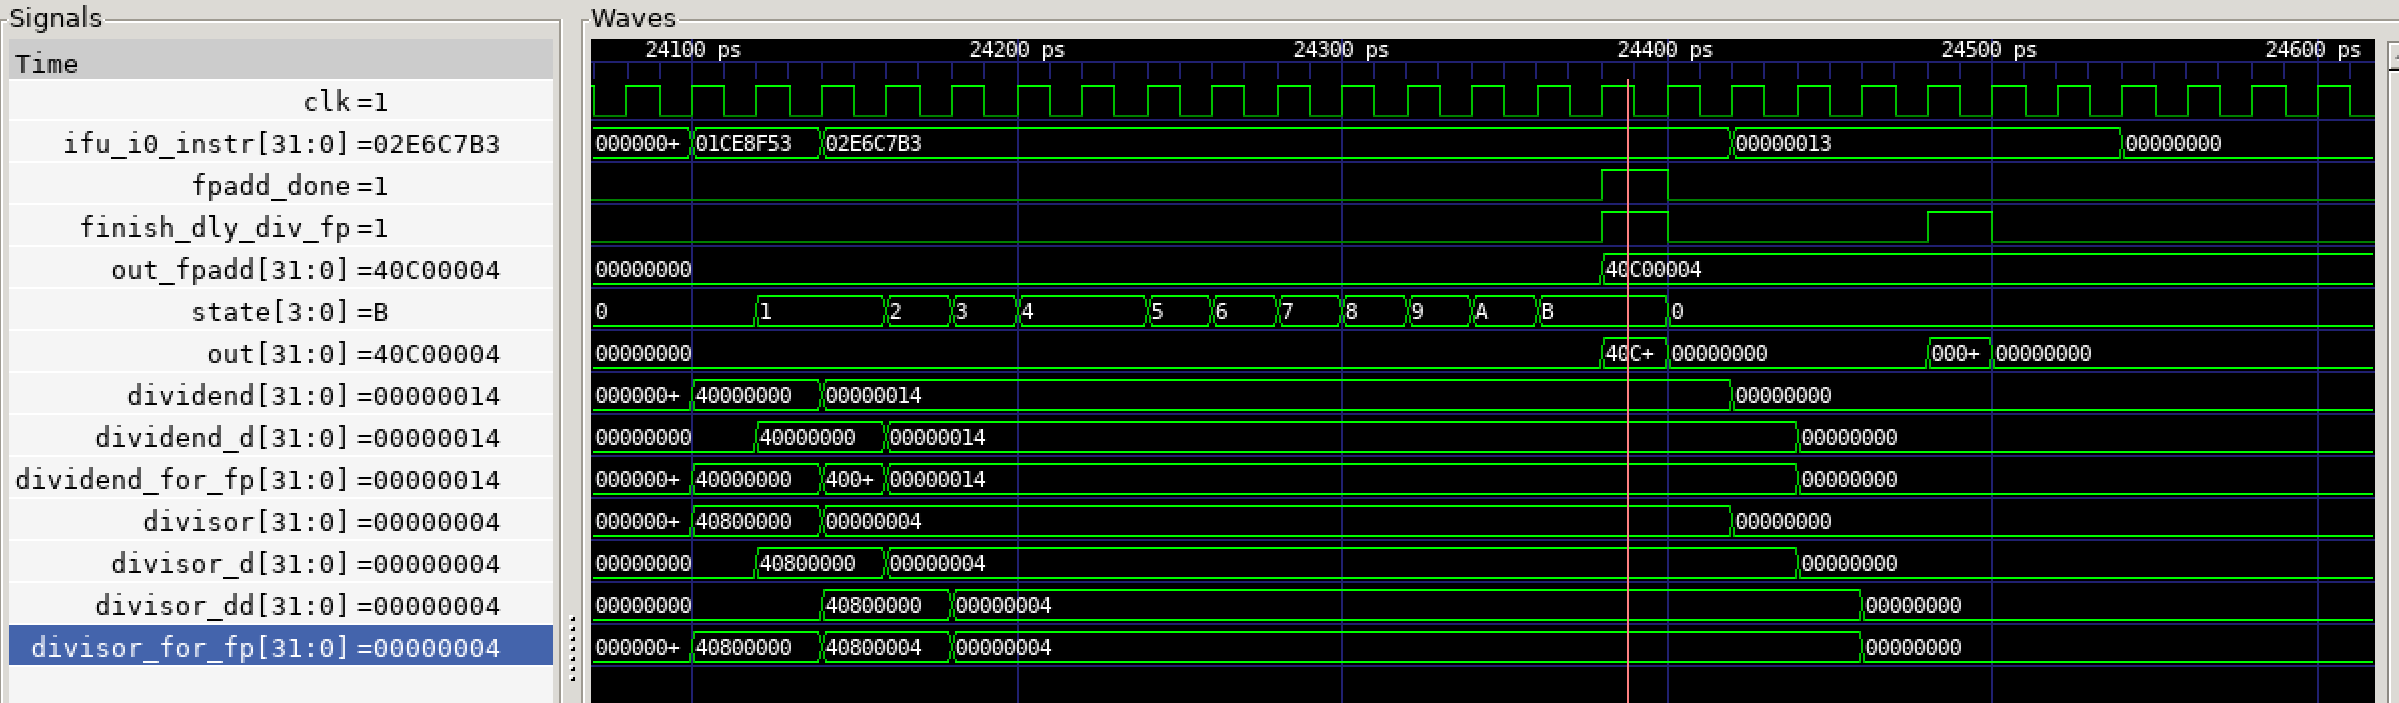
\includegraphics[width=1.0\textwidth]{ppp2.png}
    \caption{OR运算数据污染现象2}
    \label{fig:or_pollution_data}
\end{figure}

\begin{figure}[H]
    \centering
    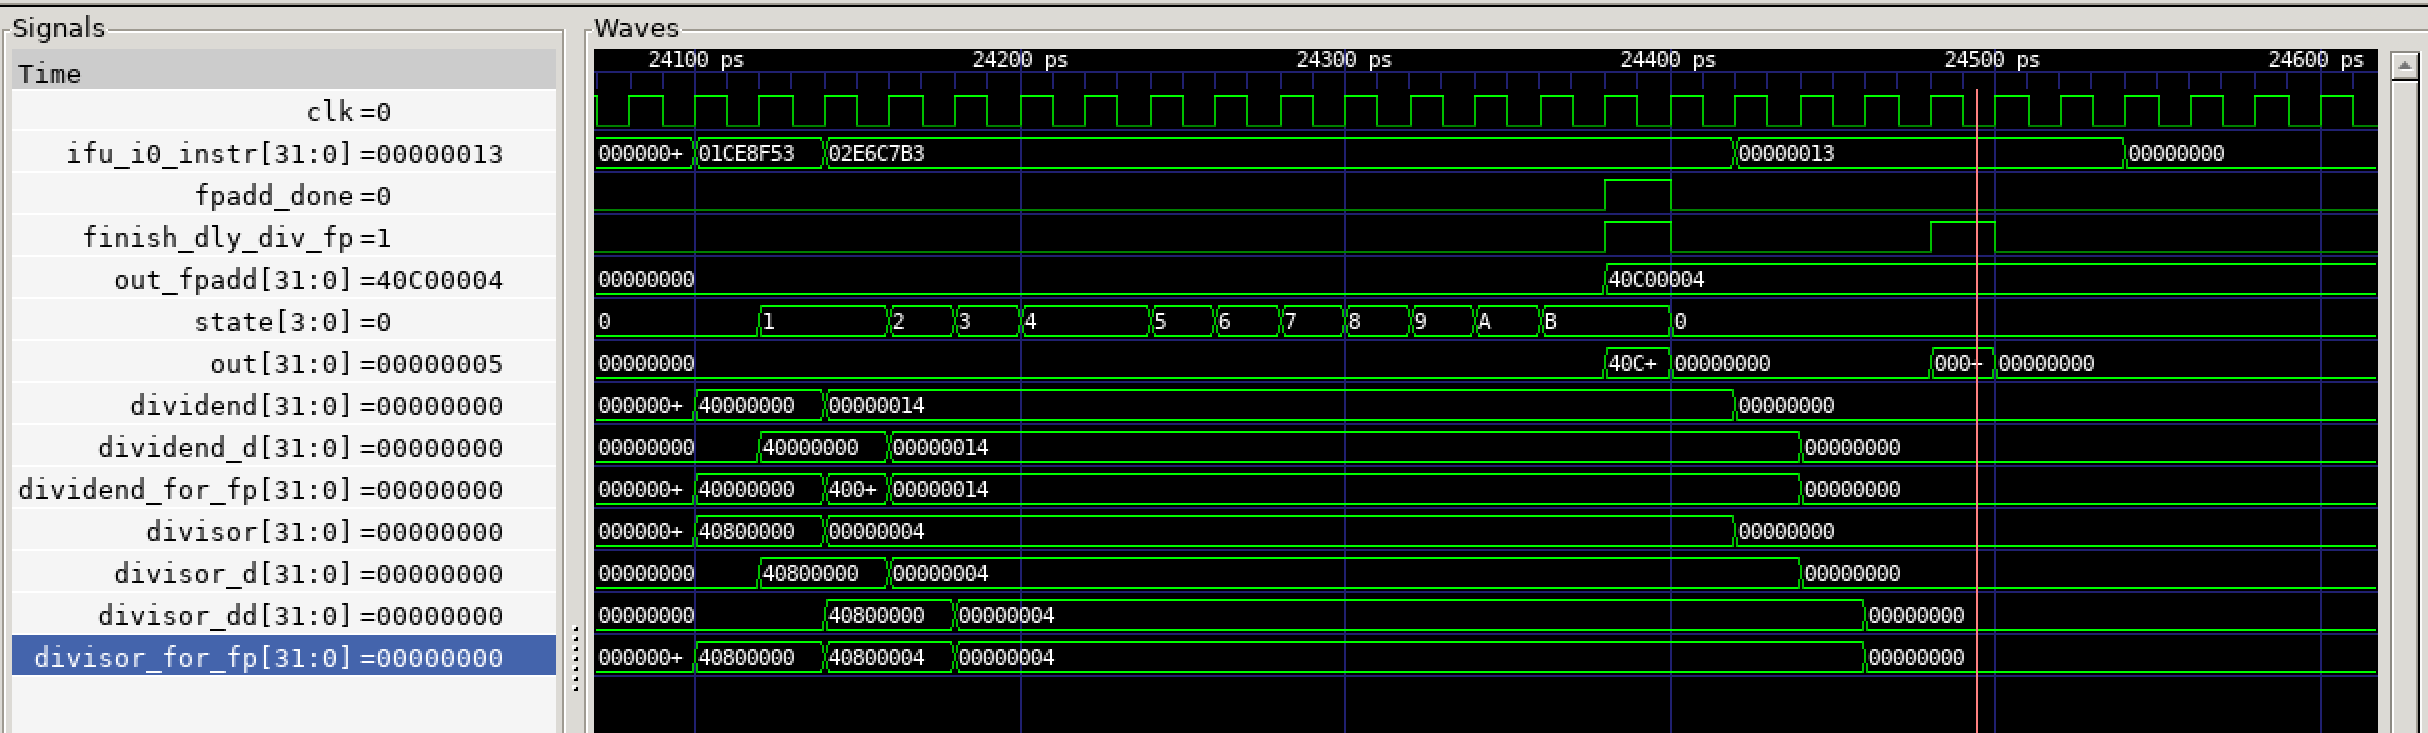
\includegraphics[width=1.0\textwidth]{ppp3.png}
    \caption{OR运算数据污染现象3}
    \label{fig:or_pollution_result}
\end{figure}

\textbf{关键信号观察}（图\ref{fig:or_pollution_state}、图\ref{fig:or_pollution_data} 和 图\ref{fig:or_pollution_result}）：

\begin{enumerate}[itemsep=0pt, parsep=3pt]
    \item \textbf{指令序列}（图\ref{fig:or_pollution_state}）：
    \begin{itemize}[itemsep=0pt, parsep=3pt]
        \item 24200ps 附近：\texttt{ifu\_i0\_instr = 0x01CE8F53}（fadd.s 指令）
        \item 24300ps 附近：\texttt{ifu\_i0\_instr = 0x02E6C7B3}（div 指令）
        \item 两条指令间隔极短，形成零延迟背靠背执行
    \end{itemize}
    
    \item \textbf{数据污染过程}（图\ref{fig:or_pollution_data}）：
    \begin{itemize}[itemsep=0pt, parsep=3pt]
        \item \textbf{初始阶段}：\texttt{divisor\_for\_fp = 0x40800000}（浮点数4.0，正确）
        \item \textbf{div指令进入后}：
        \begin{itemize}[itemsep=0pt, parsep=3pt]
            \item \texttt{divisor} 变为 \texttt{0x00000004}（整数4）
            \item \texttt{divisor\_d} 仍为 \texttt{0x40800000}（上一周期的浮点数）
            \item \texttt{divisor\_for\_fp = 0x40800000 | 0x00000004 = 0x40800004} ⚠️ 数据污染！
        \end{itemize}
        \item \textbf{后续周期}：\texttt{divisor\_for\_fp} 逐渐清零（\texttt{0x00000004 | 0x00000000}）
        \item \texttt{dividend\_for\_fp} 也出现类似污染现象
    \end{itemize}
    
    \item \textbf{计算结果错误}（图\ref{fig:or_pollution_result}）：
    \begin{itemize}[itemsep=0pt, parsep=3pt]
        \item \textbf{预期结果}：4.0 + 2.0 = 6.0 = \texttt{0x40C00000}（IEEE 754）
        \item \textbf{实际结果}：\texttt{out\_fpadd = 0x40C00004}
        \item \textbf{误差来源}：输入被污染为 \texttt{0x40800004}（≈ 4.0000047）
        \item 计算过程：$4.0000047 + 2.0 = 6.0000047 \approx$ \texttt{0x40C00004} ✓ 逻辑正确但输入错误
    \end{itemize}
    
    \item \textbf{状态机正常执行}（图\ref{fig:or_pollution_state}）：
    \begin{itemize}[itemsep=0pt, parsep=3pt]
        \item \texttt{state[3:0]} 完整经历 0→1→2→...→B（12个状态）
        \item \texttt{fpadd\_done} 在状态 B 完成后拉高
        \item \texttt{finish\_dly\_div\_fp} 正确指示运算完成
        \item 说明：\textbf{控制逻辑正确，问题仅在数据路径}
    \end{itemize}
\end{enumerate}

\subsubsection{结论}

\textbf{结论}：OR运算数据保持方案\textbf{存在缺陷}！

\textbf{问题根源}：
\begin{itemize}[itemsep=0pt, parsep=3pt]
    \item OR运算只适用于"保持非零值"的场景（数据 0 → 非零，或 非零 → 0）
    \item 当新旧数据都非零时（非零A → 非零B），OR运算会产生 A|B 的混合值
    \item 在浮点/整数连续执行场景下，这种混合值会破坏IEEE 754编码
\end{itemize}
\clearpage
\subsection{优化方案实现}

\subsubsection{初步锁存方案}

根据上一节分析，我们将OR运算方案替换为锁存方案。
\begin{lstlisting}[language=Verilog]
// 初步方案：直接在stb信号有效时锁存数据
reg [31:0] fp_operand_a;
reg [31:0] fp_operand_b;
reg stb_d, stb_dd, stb_ddd;

assign stb = fp.fp_add;

always@(posedge clk) begin
    stb_d <= stb;
    stb_dd <= stb_d;
    stb_ddd <= stb_dd;
    
    if (stb) begin  // 在stb信号有效时锁存
        fp_operand_a <= dividend;
        fp_operand_b <= divisor;
    end
end

assign stb_for_fp = stb | stb_d | stb_dd | stb_ddd;

fp_adder simple_fp_adder(
    .input_a(fp_operand_a),
    .input_b(fp_operand_b),
    .input_a_stb(stb_for_fp),
    .input_b_stb(stb_for_fp),
    // ...
);
\end{lstlisting}

然而，通过波形分析发现\textbf{握手时序问题}：fp\_adder内部的寄存器\texttt{a}始终为0，浮点运算无法正常进行。

\subsubsection{时序问题的根本原因}

通过添加fp\_adder内部信号到波形查看器，我们发现了问题的本质：

\begin{figure}[H]
    \centering
    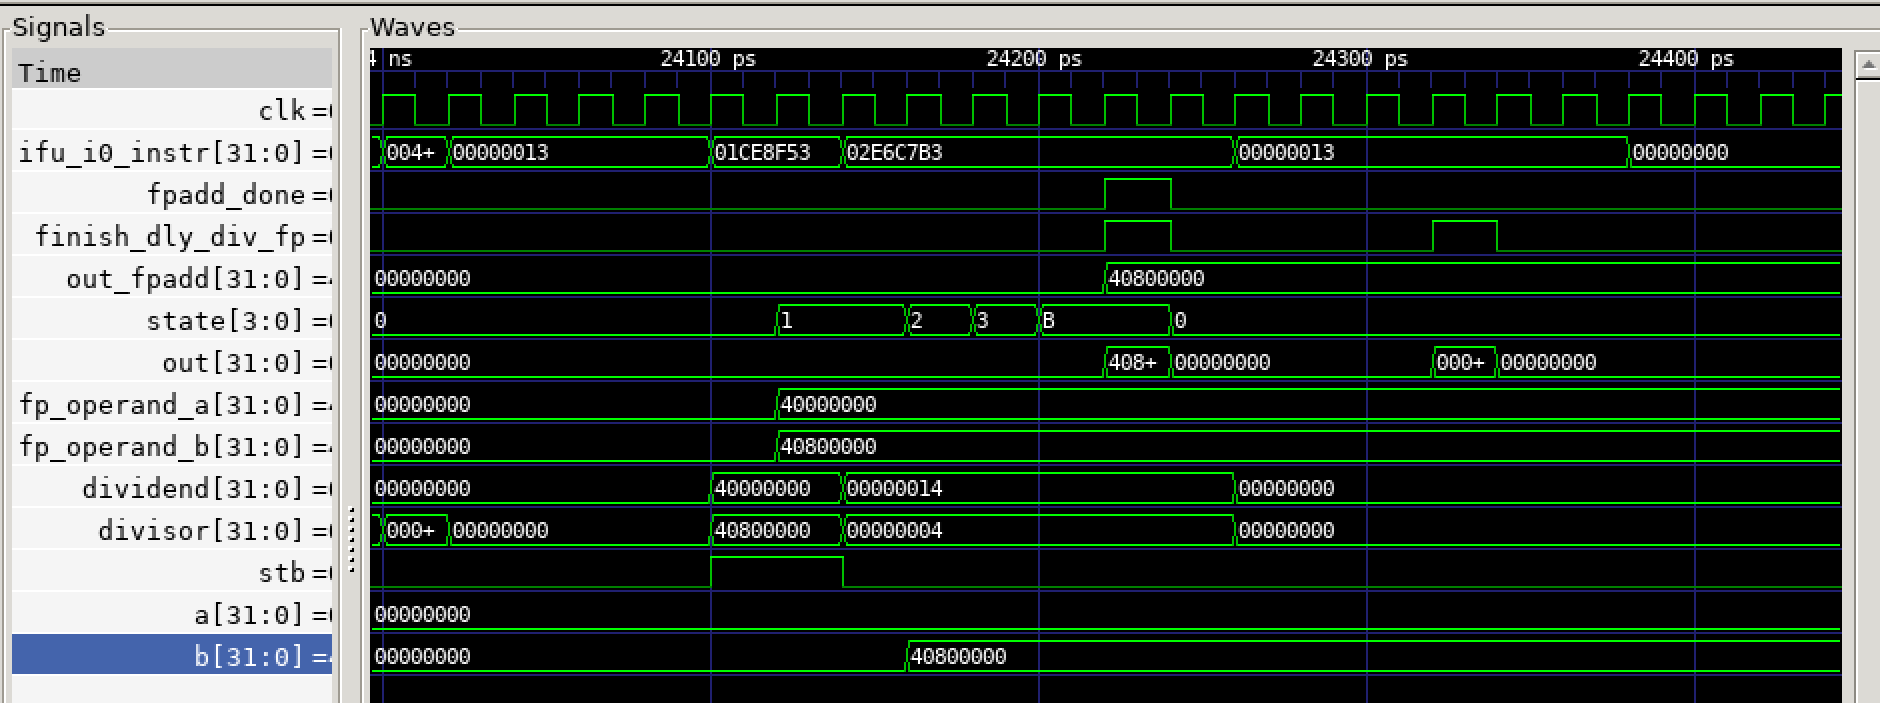
\includegraphics[width=1.0\textwidth]{pp9.png}
    \caption{握手时序问题波形分析}
    \label{fig:handshake_timing_issue}
\end{figure}

\textbf{时序冲突分析}（图\ref{fig:handshake_timing_issue}）：

\begin{itemize}[itemsep=0pt, parsep=3pt]
    \item \textbf{T0周期}（stb=1）：
    \begin{itemize}[itemsep=0pt, parsep=3pt]
        \item \texttt{fp.fp\_add} 拉高，\texttt{stb\_for\_fp = stb | stb\_d | stb\_dd | stb\_ddd} 立即变为1
        \item fp\_adder 状态机在 \texttt{get\_a} 状态，满足 \texttt{s\_input\_a\_ack \&\& input\_a\_stb}
        \item \textbf{同一时钟上升沿}：\texttt{fp\_operand\_a <= dividend} 开始执行（非阻塞赋值）
        \item \textbf{握手时刻}：fp\_adder 读取 \texttt{input\_a}，但此时 \texttt{fp\_operand\_a} 还未更新，仍为旧值0
        \item \textbf{结果}：\texttt{a <= 0}，数据采样失败
    \end{itemize}
    
    \item \textbf{T1周期}（stb\_d=1）：
    \begin{itemize}[itemsep=0pt, parsep=3pt]
        \item \texttt{fp\_operand\_a} 已更新为 \texttt{0x40000000}（正确值）
        \item 但握手已在T0完成，状态机已跳转到 \texttt{get\_b} 状态
        \item 内部寄存器 \texttt{a} 不会再更新
    \end{itemize}
\end{itemize}

\textbf{问题本质}：\textbf{非阻塞赋值的延迟特性}导致数据在握手时尚未稳定。

\subsubsection{最终优化方案}

\textbf{解决思路}：延迟握手信号，使其在数据稳定后再触发。

\textbf{关键修改}：将 \texttt{stb\_for\_fp} 中移除当前周期的 \texttt{stb}，只使用延迟后的信号：

\begin{lstlisting}[language=Verilog]
// 最终优化方案
reg [31:0] fp_operand_a;
reg [31:0] fp_operand_b;
reg stb_d, stb_dd, stb_ddd;

assign stb = fp.fp_add;

always@(posedge clk) begin
    stb_d <= stb;
    stb_dd <= stb_d;
    stb_ddd <= stb_dd;
    
    if (stb) begin  // 在stb拉高时锁存数据
        fp_operand_a <= dividend;
        fp_operand_b <= divisor;
    end
end

// 关键优化：移除stb，只使用延迟信号
assign stb_for_fp = stb_d | stb_dd | stb_ddd;

fp_adder simple_fp_adder(
    .input_a(fp_operand_a),
    .input_b(fp_operand_b),
    .input_a_stb(stb_for_fp),  // 延迟1周期后才触发握手
    .input_b_stb(stb_for_fp),
    .output_z_ack(1'b1),
    .clk(clk),
    .rst(~rst_l),
    .output_z(out_fpadd),
    .output_z_stb(fpadd_done),
    .input_a_ack(),
    .input_b_ack()
);
\end{lstlisting}

\textbf{时序改进}：

\begin{itemize}[itemsep=0pt, parsep=3pt]
    \item \textbf{T0}（stb=1）：\texttt{fp\_operand\_a/b} 开始锁存数据，\texttt{stb\_for\_fp=0}（未握手）
    \item \textbf{T1}（stb\_d=1）：\texttt{fp\_operand\_a/b} 已稳定为正确值，\texttt{stb\_for\_fp=1}（触发握手），状态机从 \texttt{get\_a} → \texttt{get\_b}
    \item \textbf{T2}（stb\_dd=1）：\texttt{stb\_for\_fp=1}（保持握手），状态机从 \texttt{get\_b} → \texttt{unpack}
    \item \textbf{T3}（stb\_ddd=1）：\texttt{stb\_for\_fp=1}（延长握手窗口），确保状态机稳定转换
\end{itemize}

\textbf{验证结果}：

\begin{figure}[H]
    \centering
    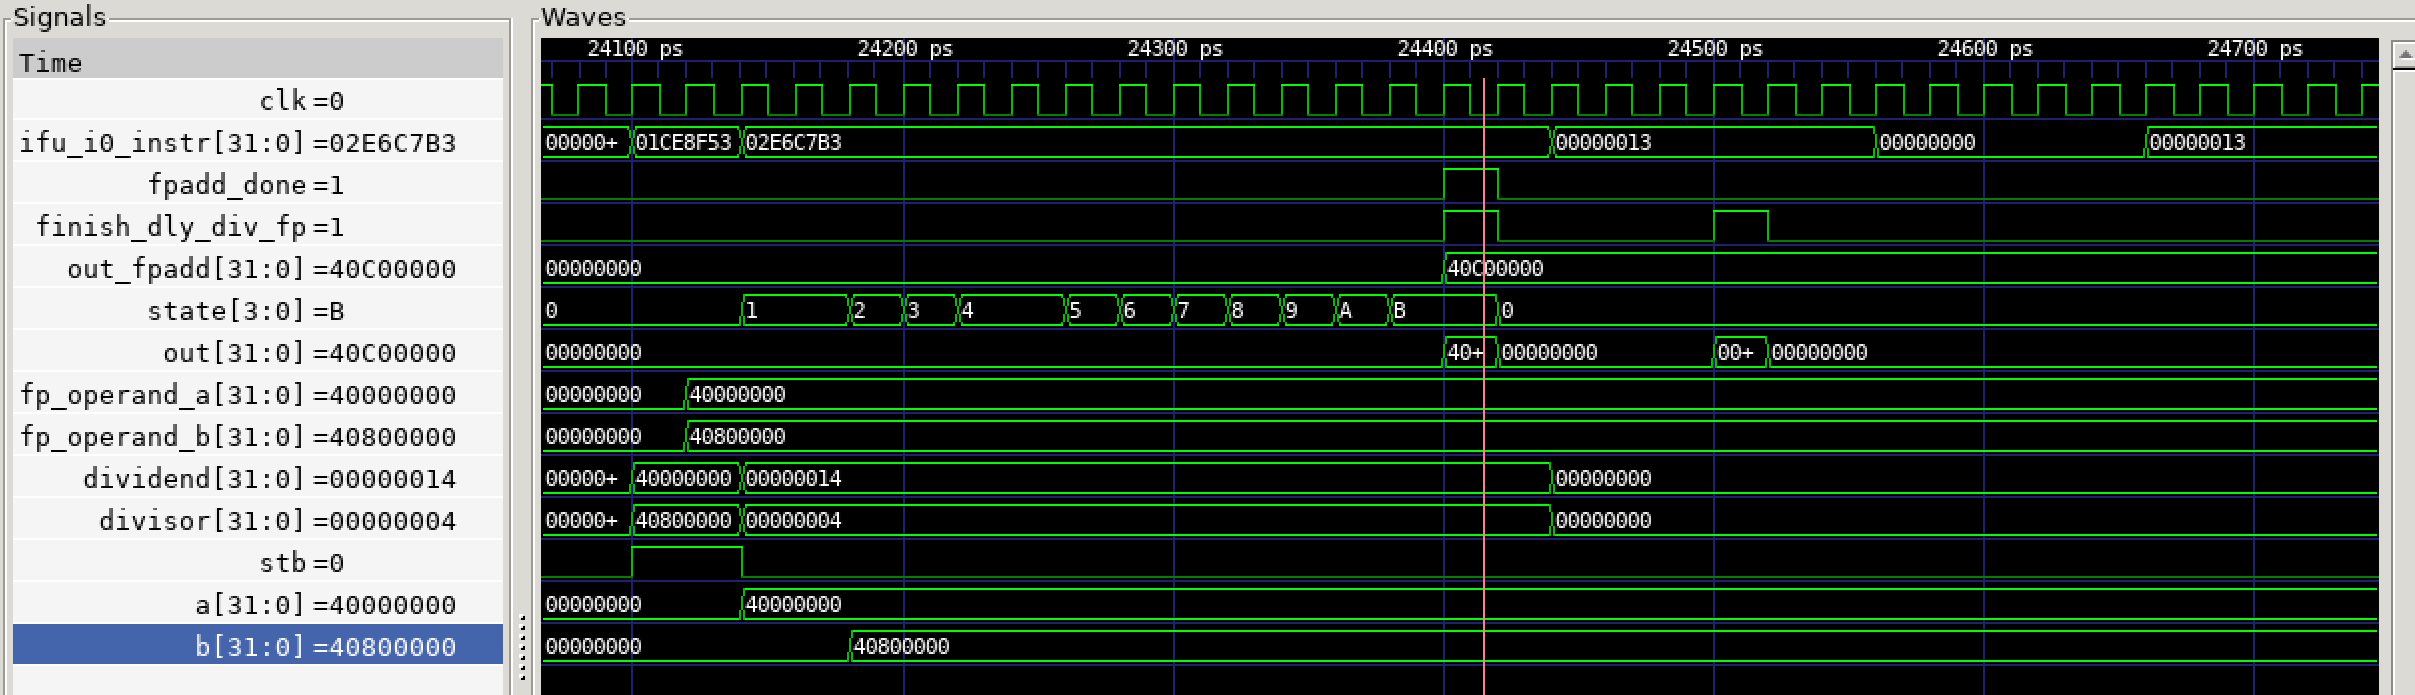
\includegraphics[width=1.0\textwidth]{pp7.png}
    \caption{优化后的正确波形1}
    \label{fig:optimized_waveform}
\end{figure}

\begin{figure}[H]
    \centering
    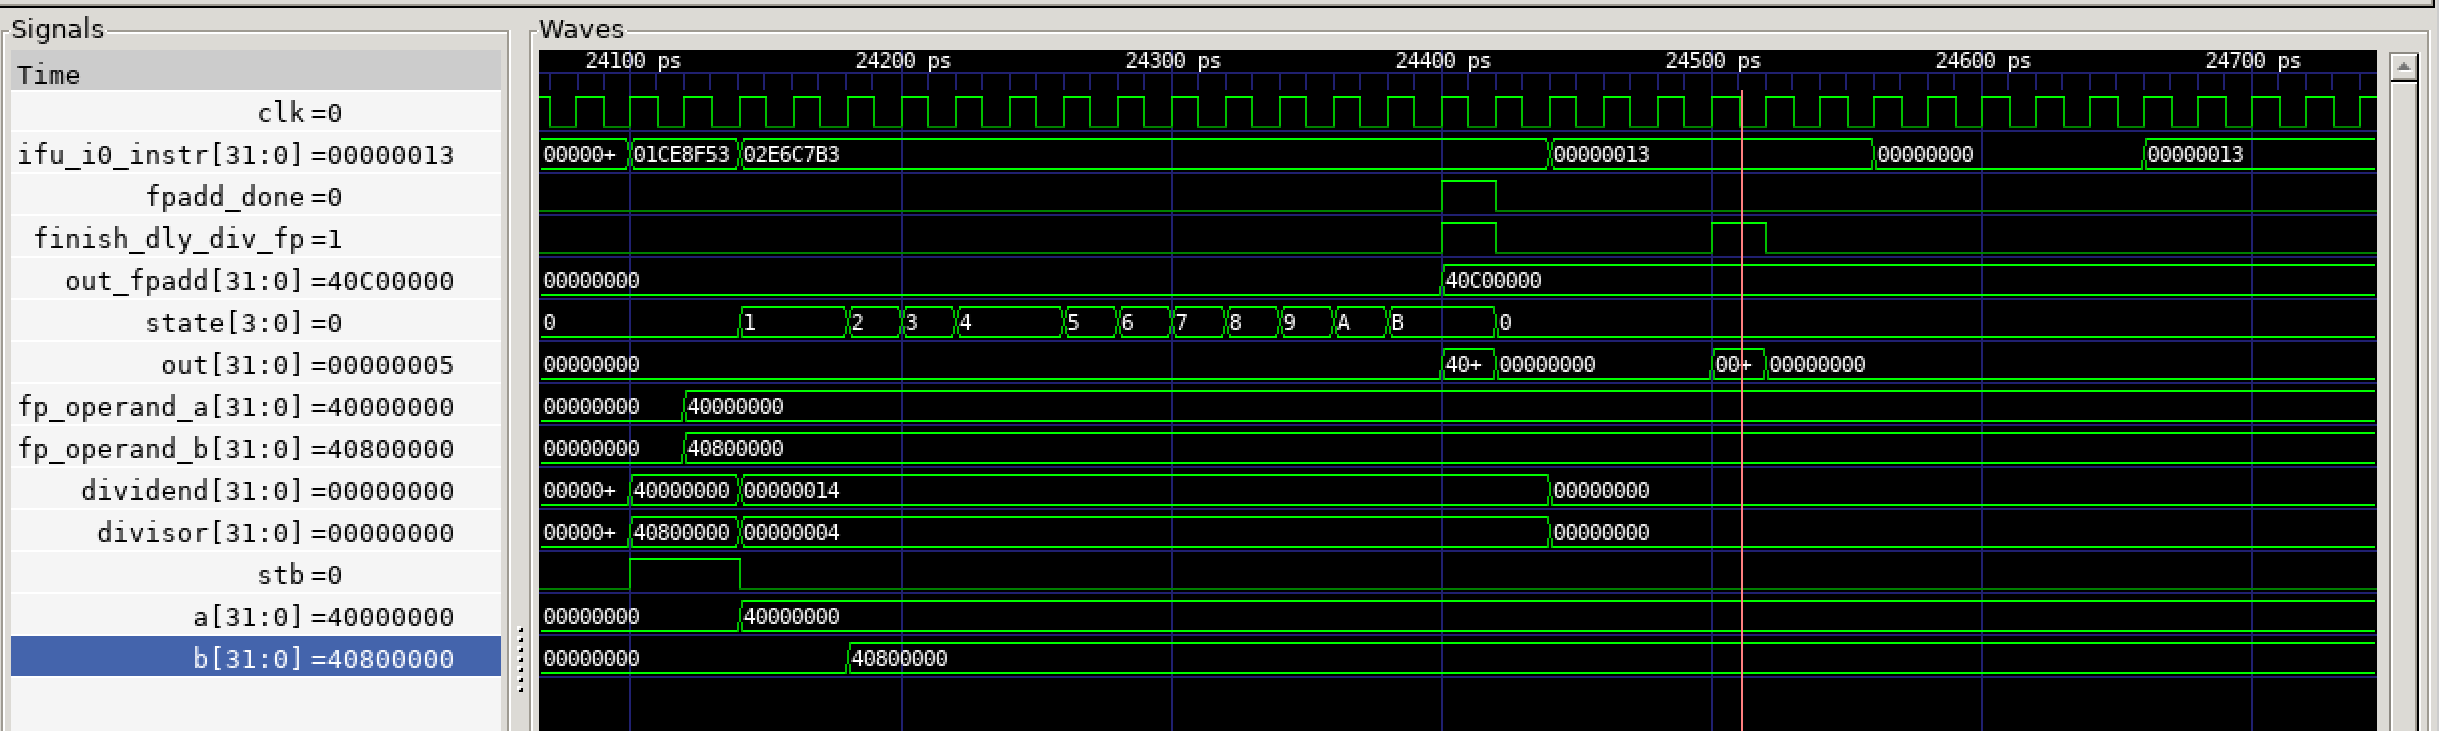
\includegraphics[width=1.0\textwidth]{pp8.png}
    \caption{优化后的正确波形2}
    \label{fig:optimized_waveform}
\end{figure}

图\ref{fig:optimized_waveform} 显示优化后的波形特征：

\begin{itemize}[itemsep=0pt, parsep=3pt]
    \item \texttt{fp\_operand\_a = 0x40000000}（2.0，正确）
    \item \texttt{fp\_operand\_b = 0x40800000}（4.0，正确）
    \item \texttt{simple\_fp\_adder.a = 0x40000000}（内部寄存器已正确锁存）
    \item \texttt{simple\_fp\_adder.b = 0x40800000}（内部寄存器已正确锁存）
    \item \texttt{out\_fpadd = 0x40C00000}（6.0，计算正确）
    \item \texttt{state[3:0]} 正常完成 0→1→2→...→B 状态转换
\end{itemize}

\textbf{方案优势总结}：

\begin{table}[H]
\centering
\begin{tabular}{|l|c|c|c|}
\hline
\textbf{特性} & \textbf{OR方案} & \textbf{初步锁存方案} & \textbf{优化锁存方案} \\
\hline
数据污染 & ✗ 存在 & ✓ 无 & ✓ 无 \\
\hline
握手时序 & ✓ 正确 & ✗ 数据未稳定 & ✓ 数据已稳定 \\
\hline
内部采样 & ✓ 成功 & ✗ 采样到0 & ✓ 成功 \\
\hline
计算结果 & ✗ 错误(污染) & ✗ 错误(数据为0) & ✓ 完全正确 \\
\hline
资源消耗 & 4寄存器 & 5寄存器 & 5寄存器 \\
\hline
\end{tabular}
\caption{三种方案对比}
\end{table}

\subsubsection{状态机握手实现}

为了更好地控制握手时序和数据同步，我们采用了基于FSM（有限状态机）的握手协议实现方案。该方案通过显式的状态转换来管理operand锁存、握手信号生成和结果接收的整个流程。

\textbf{FSM设计}：

状态机包含6个状态：
\begin{itemize}[itemsep=0pt, parsep=3pt]
    \item \texttt{FSM\_IDLE}：空闲状态，等待浮点加指令
    \item \texttt{FSM\_LATCH\_DATA}：锁存操作数到专用寄存器
    \item \texttt{FSM\_SEND\_A}：等待input\_a的ack信号，然后发送input\_a\_stb
    \item \texttt{FSM\_SEND\_B}：等待input\_b的ack信号，然后发送input\_b\_stb
    \item \texttt{FSM\_COMPUTING}：等待fp\_adder计算完成（output\_z\_stb拉高）
    \item \texttt{FSM\_COMPLETE}：标记结果有效，下周期返回IDLE
\end{itemize}

\textbf{核心代码}：

\begin{lstlisting}[language=Verilog]
// FSM状态定义
localparam [2:0] FSM_IDLE        = 3'd0,
                 FSM_LATCH_DATA  = 3'd1,
                 FSM_SEND_A      = 3'd2,
                 FSM_SEND_B      = 3'd3,
                 FSM_COMPUTING   = 3'd4,
                 FSM_COMPLETE    = 3'd5;

reg [2:0] fpadd_fsm_state;
reg [31:0] fpadd_operand_a, fpadd_operand_b;
reg fpadd_input_a_stb, fpadd_input_b_stb;
wire fpadd_input_a_ack, fpadd_input_b_ack;
wire [31:0] fpadd_result;
wire fpadd_result_valid;

// FSM状态转换逻辑
always @(posedge clk or negedge rst_l) begin
  if (!rst_l) begin
    fpadd_fsm_state <= FSM_IDLE;
    fpadd_input_a_stb <= 1'b0;
    fpadd_input_b_stb <= 1'b0;
    fpadd_operand_a <= 32'h0;
    fpadd_operand_b <= 32'h0;
  end else begin
    case (fpadd_fsm_state)
      FSM_IDLE: begin
        if (fp.fp_add) begin  // 检测到浮点加指令
          fpadd_operand_a <= dividend;  // 锁存操作数
          fpadd_operand_b <= divisor;
          fpadd_fsm_state <= FSM_LATCH_DATA;
        end
      end
      
      FSM_LATCH_DATA: begin  // 等待一个周期确保数据稳定
        fpadd_fsm_state <= FSM_SEND_A;
      end
      
      FSM_SEND_A: begin
        if (fpadd_input_a_ack) begin  // 等待ack
          fpadd_input_a_stb <= 1'b0;  // 撤销stb
          fpadd_fsm_state <= FSM_SEND_B;
        end else begin
          fpadd_input_a_stb <= 1'b1;  // 发送stb
        end
      end
      
      FSM_SEND_B: begin
        if (fpadd_input_b_ack) begin
          fpadd_input_b_stb <= 1'b0;
          fpadd_fsm_state <= FSM_COMPUTING;
        end else begin
          fpadd_input_b_stb <= 1'b1;
        end
      end
      
      FSM_COMPUTING: begin
        if (fpadd_result_valid) begin  // 等待计算完成
          fpadd_fsm_state <= FSM_COMPLETE;
        end
      end
      
      FSM_COMPLETE: begin
        fpadd_fsm_state <= FSM_IDLE;  // 返回空闲状态
      end
    endcase
  end
end

// 实例化fp_adder模块
fp_adder simple_fp_adder(
  .input_a(fpadd_operand_a),
  .input_b(fpadd_operand_b),
  .input_a_stb(fpadd_input_a_stb),
  .input_b_stb(fpadd_input_b_stb),
  .output_z_ack(1'b1),
  .clk(clk),
  .rst(~rst_l),
  .output_z(fpadd_result),
  .output_z_stb(fpadd_result_valid),
  .input_a_ack(fpadd_input_a_ack),
  .input_b_ack(fpadd_input_b_ack)
);
\end{lstlisting}

\textbf{FSM方案的优势}：

\begin{itemize}[itemsep=0pt, parsep=3pt]
    \item \textbf{数据隔离}：通过\texttt{FSM\_LATCH\_DATA}状态确保操作数在专用寄存器中稳定
    \item \textbf{握手清晰}：显式的ack检测和stb控制，避免时序竞争
    \item \textbf{易扩展}：可方便地添加新的浮点操作（乘法、除法等）
    \item \textbf{易调试}：状态机状态可直接在波形中观察
\end{itemize}

\textbf{测试波形}：

\begin{figure}[H]
    \centering
    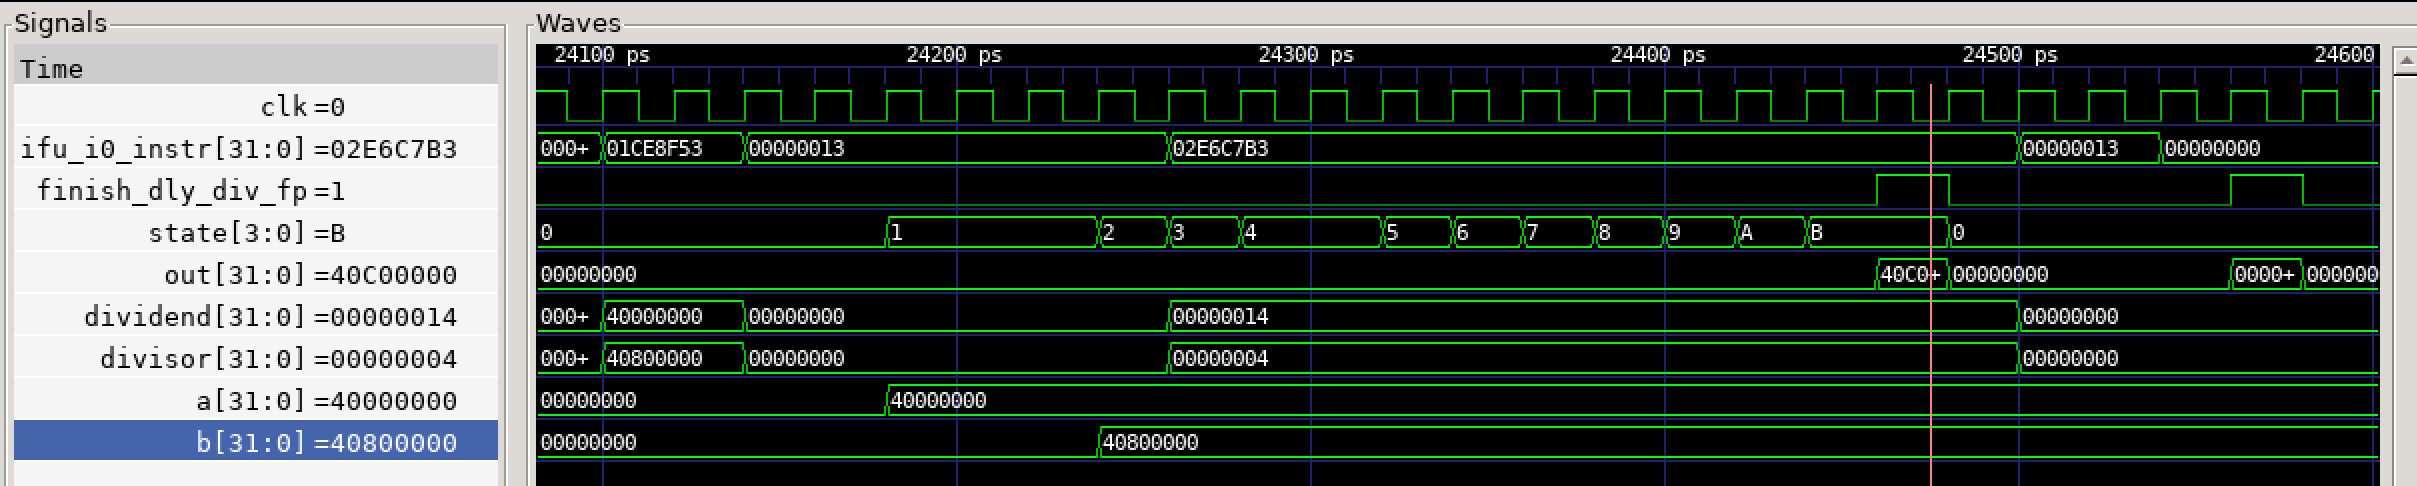
\includegraphics[width=1.0\textwidth]{adder1.png}
    \caption{FSM握手实现波形1}
    \label{fig:fsm_adder1}
\end{figure}

\begin{figure}[H]
    \centering
    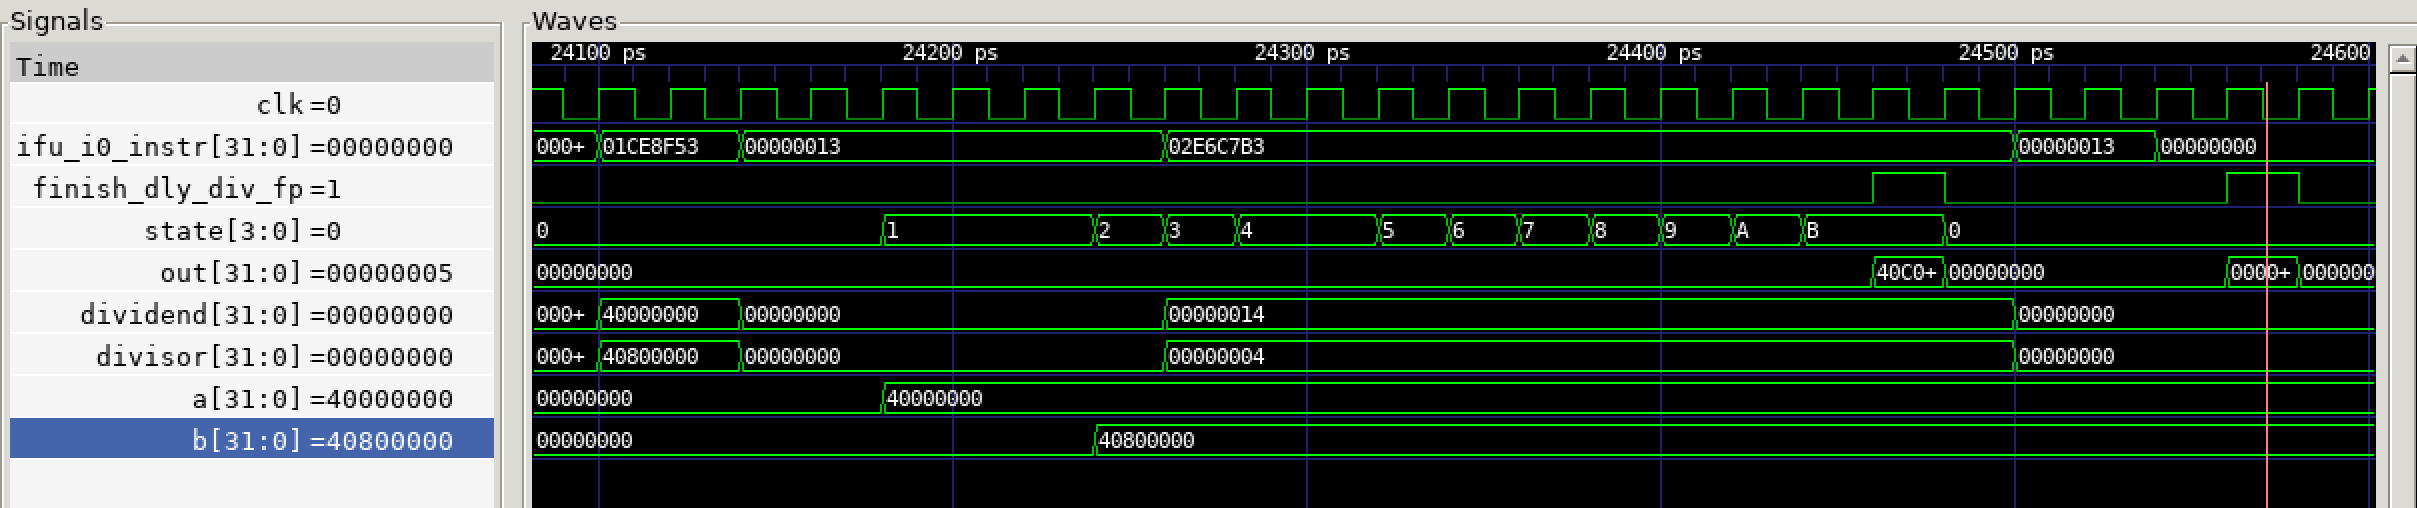
\includegraphics[width=1.0\textwidth]{adder2.png}
    \caption{FSM握手实现波形2}
    \label{fig:fsm_adder2}
\end{figure}

图\ref{fig:fsm_adder1}和图\ref{fig:fsm_adder2}展示了FSM方案的波形特征：
\begin{itemize}[itemsep=0pt, parsep=3pt]
    \item 状态机从IDLE(0) → LATCH\_DATA(1) → SEND\_A(2) → SEND\_B(3) → COMPUTING(4) → COMPLETE(5) 顺序转换
    \item 操作数在LATCH\_DATA状态锁存：\texttt{fpadd\_operand\_a = 0x40000000}（2.0），\texttt{fpadd\_operand\_b = 0x40800000}（4.0）
    \item 握手信号时序正确：\texttt{fpadd\_input\_a\_stb}和\texttt{fpadd\_input\_b\_stb}在对应状态拉高，等待ack后撤销
    \item 计算结果正确：\texttt{fpadd\_result = 0x40C00000}（6.0 = 2.0 + 4.0）
\end{itemize}

\clearpage
\subsection{乘除法器实现}

在成功实现浮点加法器的基础上，我们进一步扩展了对浮点乘法（fmul.s）和浮点除法（fdiv.s）指令的支持。硬件模块来自开源项目\texttt{https://github.com/dawsonjon/fpu}。

\subsubsection{测试代码设计}

\textbf{浮点乘法测试代码（fp\_mul.S）}：

\begin{lstlisting}[language={[x86masm]Assembler}]
#define INSERT_NOPS_1      nop;
#define INSERT_NOPS_2      nop; INSERT_NOPS_1
#define INSERT_NOPS_3      nop; INSERT_NOPS_2
#define INSERT_NOPS_4      nop; INSERT_NOPS_3
// ...
#define INSERT_NOPS_10     nop; INSERT_NOPS_9

.globl main 
main:
li t3, 0x40800000  # 4.0
li t4, 0x40000000  # 2.0
li a3, 20 
li a4, 4 
REPEAT: 
INSERT_NOPS_4 
.word 0x11ce8f53 # fmul.s f30, f29, f28 (2.0 * 4.0 = 8.0)
INSERT_NOPS_4  
div a5, a3, a4      # 验证整数除法仍正常工作
INSERT_NOPS_10 
beq zero, zero, REPEAT
\end{lstlisting}

\textbf{指令编码说明}：
\begin{itemize}[itemsep=0pt, parsep=3pt]
    \item \texttt{0x11ce8f53}：fmul.s指令的机器码
    \item rs1=f29（t4，值为2.0），rs2=f28（t3，值为4.0），rd=f30
    \item 预期结果：\texttt{f30 = 2.0 * 4.0 = 8.0 = 0x41000000}
\end{itemize}
\clearpage
\textbf{浮点除法测试代码（fp\_div.S）}：

\begin{lstlisting}[language={[x86masm]Assembler}]
.globl main 
main:
li t3, 0x40800000  # 4.0
li t4, 0x40000000  # 2.0
li a3, 20 
li a4, 4 
REPEAT: 
INSERT_NOPS_4 
.word 0x19ce8f53 # fdiv.s f30, f29, f28 (2.0 / 4.0 = 0.5)
INSERT_NOPS_4  
div a5, a3, a4
INSERT_NOPS_10 
beq zero, zero, REPEAT
\end{lstlisting}

\textbf{指令编码说明}：
\begin{itemize}[itemsep=0pt, parsep=3pt]
    \item \texttt{0x19ce8f53}：fdiv.s指令的机器码
    \item rs1=f29（t4，值为2.0被除数），rs2=f28（t3，值为4.0除数），rd=f30
    \item 预期结果：\texttt{f30 = 2.0 / 4.0 = 0.5 = 0x3F000000}
\end{itemize}

\subsubsection{状态机集成过程}

乘法器和除法器采用与加法器相同的FSM握手方案。在\texttt{el2\_exu\_div\_ctl.sv}中，我们为每个浮点操作创建了独立的FSM实例：

\begin{lstlisting}[language=Verilog]
// 浮点乘法FSM
reg [2:0] fpmul_fsm_state;
reg [31:0] fpmul_operand_a, fpmul_operand_b;
reg fpmul_input_a_stb, fpmul_input_b_stb;
wire fpmul_result_valid;
wire [31:0] fpmul_result;

// 浮点除法FSM
reg [2:0] fpdiv_fsm_state;
reg [31:0] fpdiv_operand_a, fpdiv_operand_b;
reg fpdiv_input_a_stb, fpdiv_input_b_stb;
wire fpdiv_result_valid;
wire [31:0] fpdiv_result;

// 乘法FSM状态转换（与加法类似）
always @(posedge clk or negedge rst_l) begin
  if (!rst_l) begin
    fpmul_fsm_state <= FSM_IDLE;
    // ...
  end else begin
    case (fpmul_fsm_state)
      FSM_IDLE: begin
        if (fp.fp_mul) begin  // 检测乘法指令
          fpmul_operand_a <= dividend;
          fpmul_operand_b <= divisor;
          fpmul_fsm_state <= FSM_LATCH_DATA;
        end
      end
      // ... 其他状态与加法FSM一致
    endcase
  end
end

// 除法FSM状态转换（结构相同）
always @(posedge clk or negedge rst_l) begin
  if (!rst_l) begin
    fpdiv_fsm_state <= FSM_IDLE;
    // ...
  end else begin
    case (fpdiv_fsm_state)
      FSM_IDLE: begin
        if (fp.fp_div) begin  // 检测除法指令
          fpdiv_operand_a <= dividend;
          fpdiv_operand_b <= divisor;
          fpdiv_fsm_state <= FSM_LATCH_DATA;
        end
      end
      // ...
    endcase
  end
end

// 实例化乘法器
multiplier simple_fp_multiplier(
  .input_a(fpmul_operand_a),
  .input_b(fpmul_operand_b),
  .input_a_stb(fpmul_input_a_stb),
  .input_b_stb(fpmul_input_b_stb),
  .output_z_ack(1'b1),
  .clk(clk),
  .rst(~rst_l),
  .output_z(fpmul_result),
  .output_z_stb(fpmul_result_valid),
  .input_a_ack(fpmul_input_a_ack),
  .input_b_ack(fpmul_input_b_ack)
);

// 实例化除法器
divider simple_fp_divider(
  .input_a(fpdiv_operand_a),
  .input_b(fpdiv_operand_b),
  .input_a_stb(fpdiv_input_a_stb),
  .input_b_stb(fpdiv_input_b_stb),
  .output_z_ack(1'b1),
  .clk(clk),
  .rst(~rst_l),
  .output_z(fpdiv_result),
  .output_z_stb(fpdiv_result_valid),
  .input_a_ack(fpdiv_input_a_ack),
  .input_b_ack(fpdiv_input_b_ack)
);
\end{lstlisting}

\textbf{输出选择逻辑}：

为了支持4种操作（整数除法、浮点加/乘/除），我们使用one-hot编码的\texttt{active\_operation[3:0]}信号来选择输出：

\begin{lstlisting}[language=Verilog]
// active_operation[3]=整数除法, [2]=浮点加, [1]=浮点乘, [0]=浮点除
assign finish_dly_div_fp = ({32{active_operation[3]}} & {32{finish_dly}}) |
                           ({32{active_operation[2]}} & {32{fpadd_result_valid}}) |
                           ({32{active_operation[1]}} & {32{fpmul_result_valid}}) |
                           ({32{active_operation[0]}} & {32{fpdiv_result_valid}});

assign out_div_fp[31:0] = ({32{active_operation[3]}} & out[31:0]) |
                          ({32{active_operation[2]}} & fpadd_result[31:0]) |
                          ({32{active_operation[1]}} & fpmul_result[31:0]) |
                          ({32{active_operation[0]}} & fpdiv_result[31:0]);
\end{lstlisting}

\subsubsection{测试波形分析}

\textbf{浮点乘法波形}：

\begin{figure}[H]
    \centering
    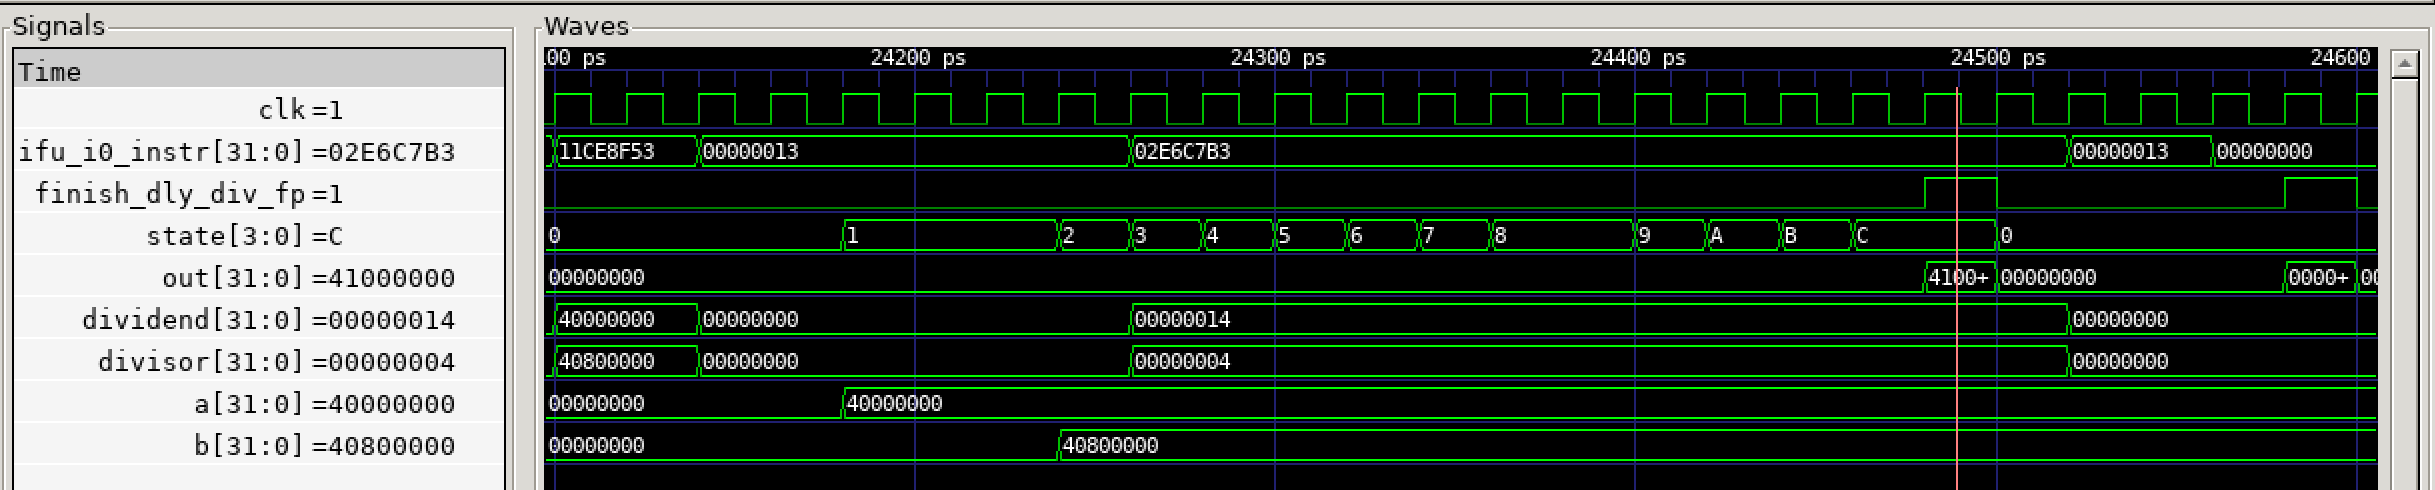
\includegraphics[width=1.0\textwidth]{mul1.png}
    \caption{浮点乘法波形1}
    \label{fig:mul1}
\end{figure}

\begin{figure}[H]
    \centering
    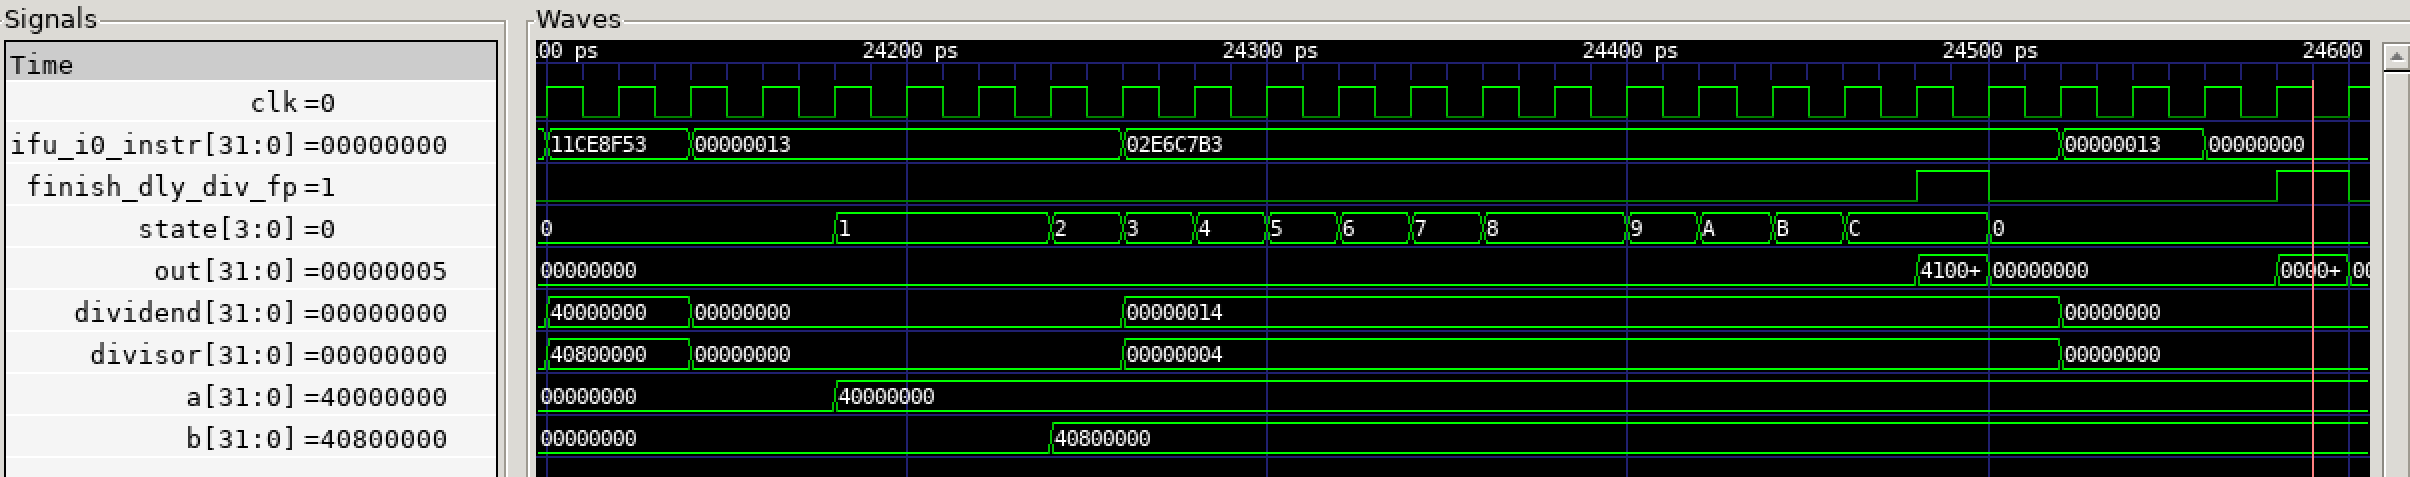
\includegraphics[width=1.0\textwidth]{mul2.png}
    \caption{浮点乘法波形2}
    \label{fig:mul2}
\end{figure}

图\ref{fig:mul1}和图\ref{fig:mul2}显示：
\begin{itemize}[itemsep=0pt, parsep=3pt]
    \item \textbf{操作数}：\texttt{fpmul\_operand\_a = 0x40000000}（2.0），\texttt{fpmul\_operand\_b = 0x40800000}（4.0）
    \item \textbf{结果}：\texttt{fpmul\_result = 0x41000000}
    \item \textbf{验证}：\texttt{0x41000000}的IEEE 754表示为$1.0 \times 2^{129-127} = 1.0 \times 2^2 = 4.0 \times 2.0 = 8.0$ ✓
\end{itemize}

\textbf{浮点除法波形}：

\begin{figure}[H]
    \centering
    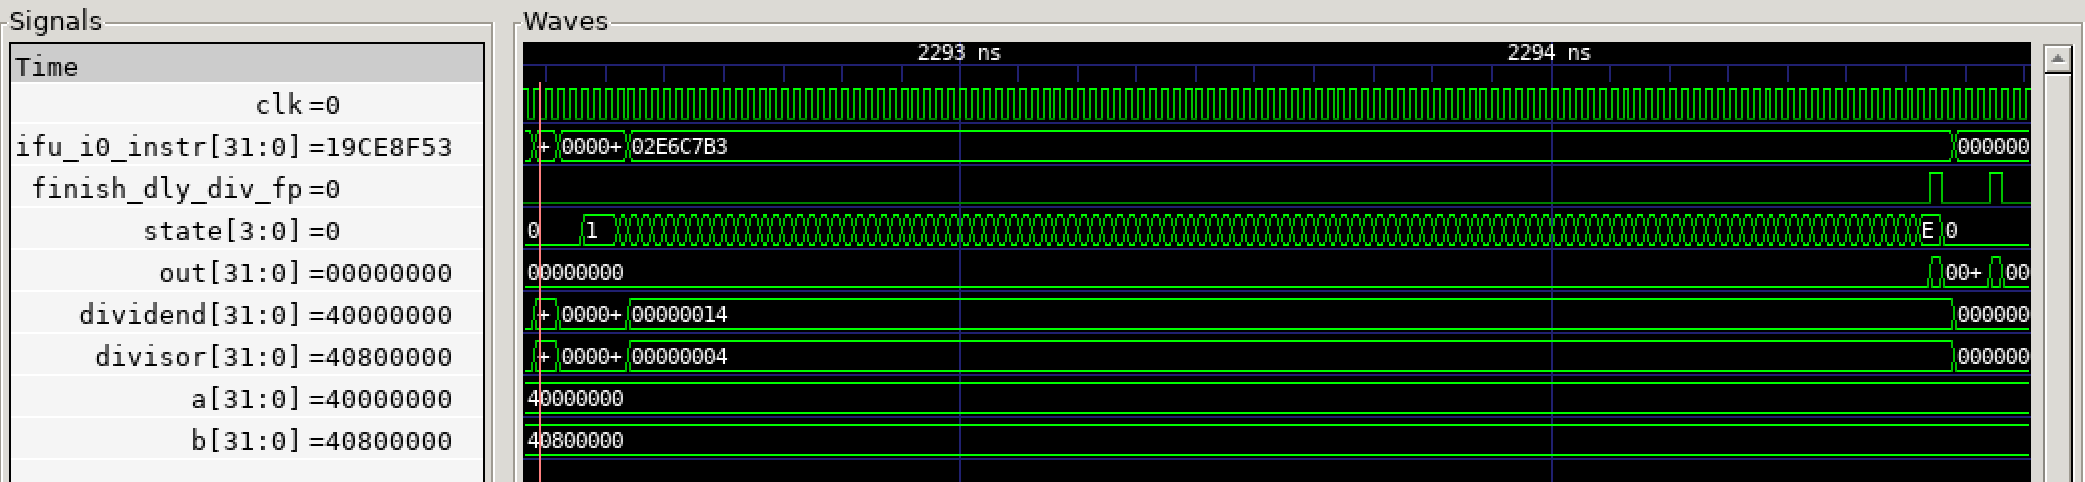
\includegraphics[width=1.0\textwidth]{div1.png}
    \caption{浮点除法波形1：迭代除法过程}
    \label{fig:div1}
\end{figure}

\begin{figure}[H]
    \centering
    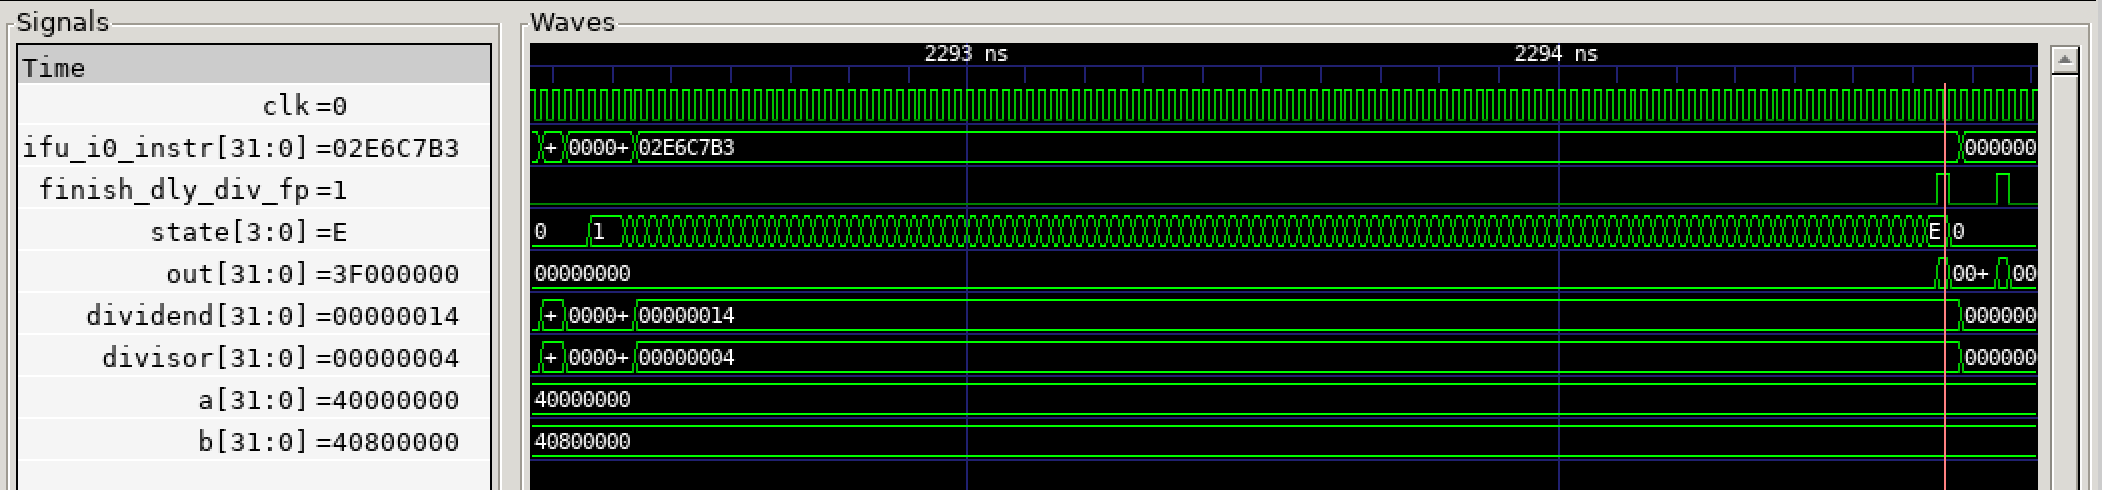
\includegraphics[width=1.0\textwidth]{div2.png}
    \caption{浮点除法波形2：状态机循环}
    \label{fig:div2}
\end{figure}

\begin{figure}[H]
    \centering
    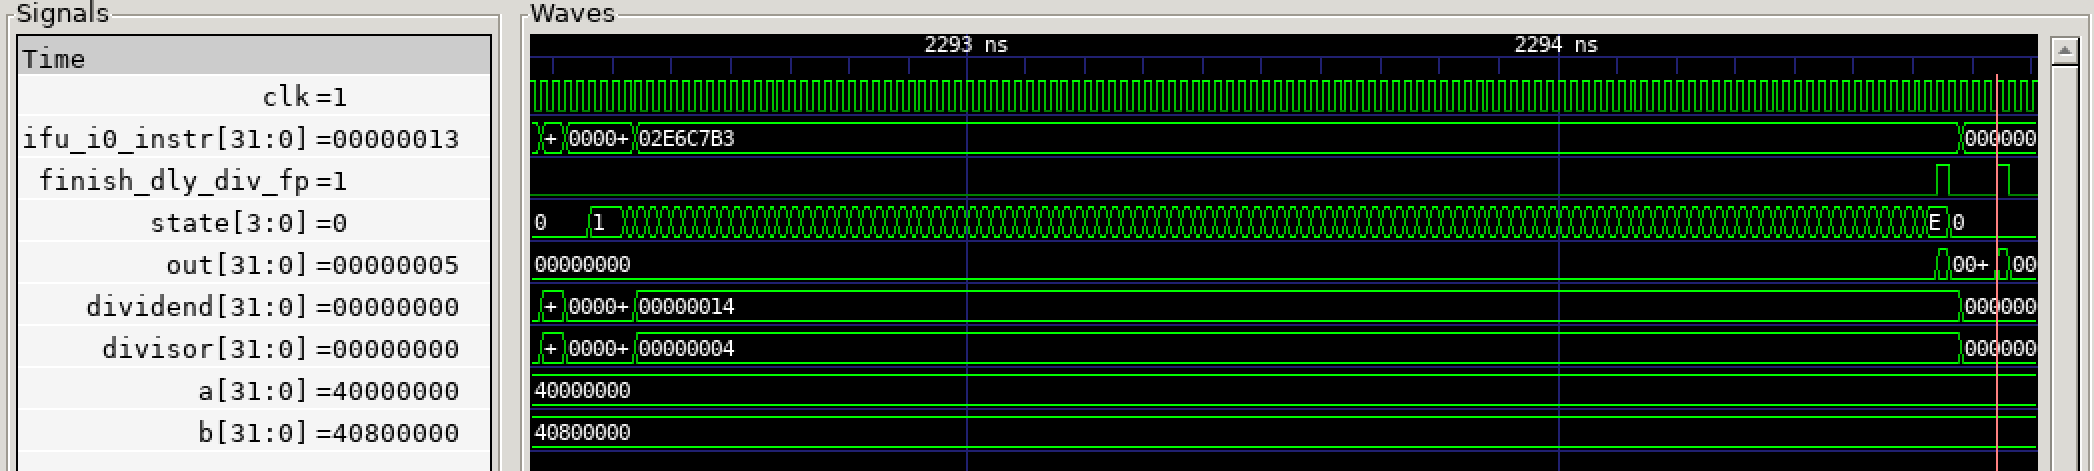
\includegraphics[width=1.0\textwidth]{div3.png}
    \caption{浮点除法波形3：计算结果输出}
    \label{fig:div3}
\end{figure}

图\ref{fig:div1}、图\ref{fig:div2}和图\ref{fig:div3}显示：
\begin{itemize}[itemsep=0pt, parsep=3pt]
    \item \textbf{操作数}：\texttt{fpdiv\_operand\_a = 0x40000000}（2.0被除数），\texttt{fpdiv\_operand\_b = 0x40800000}（4.0除数）
    \item \textbf{除法器特性}：内部状态机在state=7（divide\_1）和state=8（divide\_2）之间迭代50次完成除法运算
    \item \textbf{结果}：\texttt{fpdiv\_result = 0x3F000000}
    \item \textbf{验证}：\texttt{0x3F000000}的IEEE 754表示为符号位0，指数126（实际-1），尾数0，值为$1.0 \times 2^{-1} = 0.5 = 2.0 / 4.0$ ✓
    \item \textbf{FSM状态}：外层FSM（我们的集成）和内层FSM（除法器内部）协同工作，完成完整除法流程
\end{itemize}

\clearpage
\section{遇到的问题与解决}

\subsection{Verilator编译时序错误}

\subsubsection{问题描述}

在 \pathbox{Simulators/verilatorSIM\_Trace} 目录下执行 \keyblue{make} 命令编译仿真文件时，出现编译失败，退出码为2：

\begin{lstlisting}[language=bash]
Exit Code: 2
%Error-NEEDTIMINGOPT: ptc_top.v: ...
%Error-NEEDTIMINGOPT: gpio_top.v: ...
\end{lstlisting}

\subsubsection{问题分析}

由报错代码可知，错误主要出现在以下外设模块中：
\begin{itemize}[itemsep=0pt, parsep=3pt]
    \item \texttt{ptc\_top.v} - PTC（Programmable Timer Counter）定时器模块
    \item \texttt{gpio\_top.v} - GPIO（General Purpose Input/Output）通用输入输出模块
\end{itemize}



这些Verilog文件使用了\textbf{延迟语句}（timing control），例如 \texttt{\#1}、\texttt{\#10} 等时序控制语句。而Verilator 5.x版本对时序控制有更严格的要求，必须明确指定如何处理这些时序语句，否则会报错 \texttt{NEEDTIMINGOPT}。

延迟语句示例：
\begin{lstlisting}[language=Verilog]
always @(posedge clk) begin
    #1 data_out <= data_in;  // 这种延迟语句在Verilator 5.x中需要特殊处理
end
\end{lstlisting}


\begin{itemize}[itemsep=0pt, parsep=3pt]
    \item Verilator 4.x：对延迟语句处理较为宽松，可能自动忽略
    \item Verilator 5.x：要求显式指定时序处理选项，增强了时序安全性
\end{itemize}

\subsubsection{解决方案}

修改 \pathbox{Simulators/verilatorSIM\_Trace/Makefile} 文件，在 \texttt{VERILATOR\_OPTIONS} 中添加 \texttt{--no-timing} 选项：

\begin{lstlisting}[language=make]
# 原始配置
VERILATOR_OPTIONS = --trace --timing

# 修改后配置
VERILATOR_OPTIONS = --trace --timing --no-timing
\end{lstlisting}

或者直接设置为：

\begin{lstlisting}[language=make]
VERILATOR_OPTIONS = --trace --no-timing
\end{lstlisting}

\textbf{选项说明：}
\begin{itemize}[itemsep=0pt, parsep=3pt]
    \item \texttt{--no-timing}：禁用时序模拟，忽略Verilog代码中的延迟语句
    \item \texttt{--trace}：启用波形跟踪，生成VCD文件
\end{itemize}

\subsubsection{解决结果}

添加 \texttt{--no-timing} 选项后，重新执行 \keyblue{make} 命令：

\begin{lstlisting}[language=bash]
cd /home/xzz/COD_Project/Project1/RVfpga_NexysA7-DDR/Simulators/verilatorSIM_Trace
make
\end{lstlisting}

编译成功，终端输出：
\begin{lstlisting}[language=bash]
Terminal: bash
Last Command: make
Cwd: /home/xzz/COD_Project/Project1/RVfpga_NexysA7-DDR/Simulators/verilatorSIM_Trace
Exit Code: 0
\end{lstlisting}

\textbf{验证}：成功生成可执行文件 \pathbox{verilatorSIM\_Trace/Vrvfpgasim}，可以正常运行仿真。

\clearpage
\subsection{浮点寄存器初始化错误}

\subsubsection{问题发现}

在最初测试浮点加法器时，我们使用了以下代码（\texttt{fp\_conflict\_bak.S}）：

\begin{lstlisting}[language={[x86masm]Assembler}]
main:
    li t0, 0x40000000   # t0 (x5) = 2.0
    li t1, 0x40400000   # t1 (x6) = 3.0
    li a0, 20
    li a1, 4

CRITICAL_TEST:
    INSERT_NOPS_2
    .word 0x001080d3    # fadd.s f1, f1, f0
    div a2, a0, a1
    INSERT_NOPS_20
\end{lstlisting}

运行仿真后，波形显示出现异常结果。

\begin{figure}[H]
    \centering
    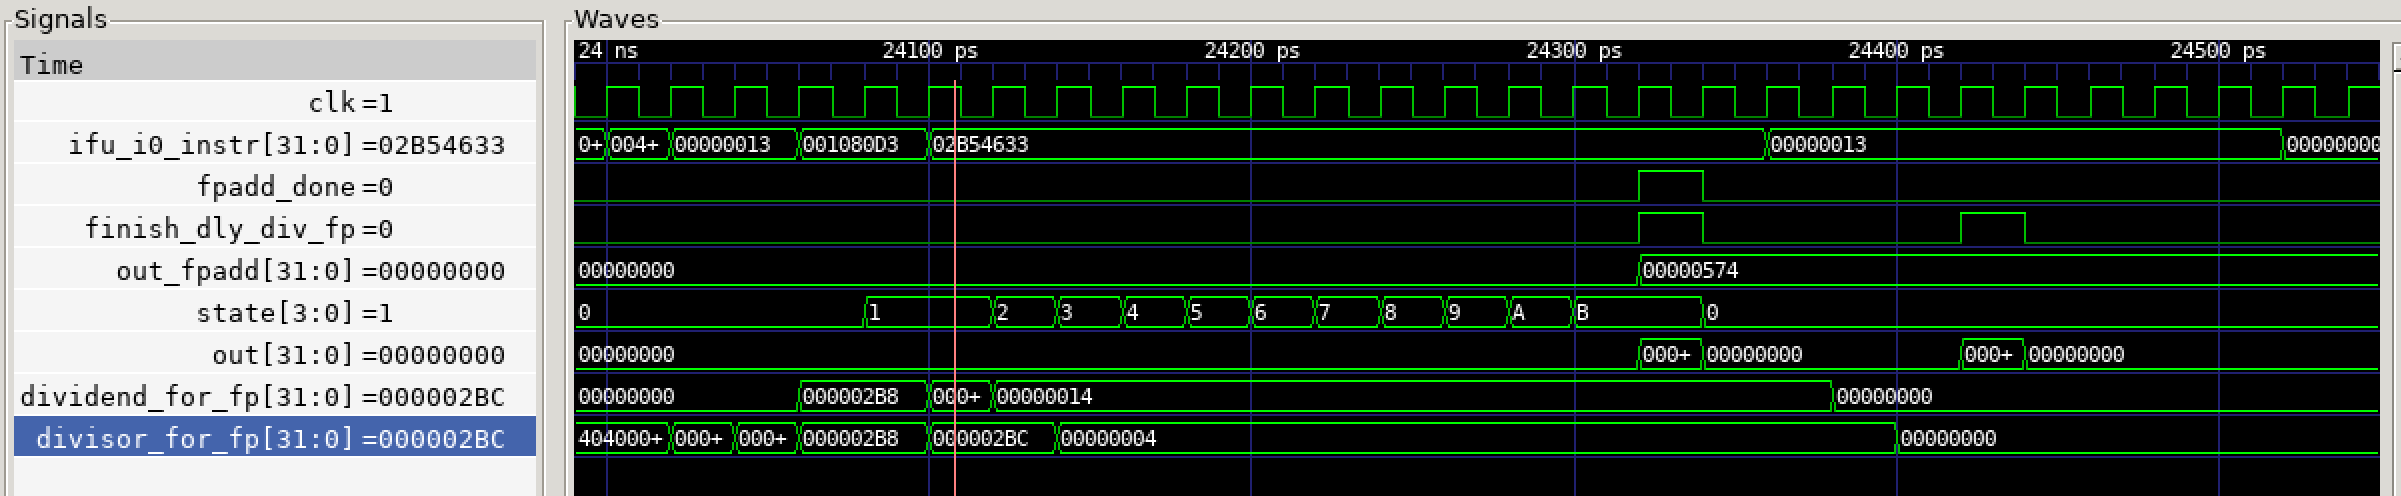
\includegraphics[width=1.0\textwidth]{pp4.png}
    \caption{错误的浮点寄存器初始化波形1}
    \label{fig:reg_init_error_state}
\end{figure}

\begin{figure}[H]
    \centering
    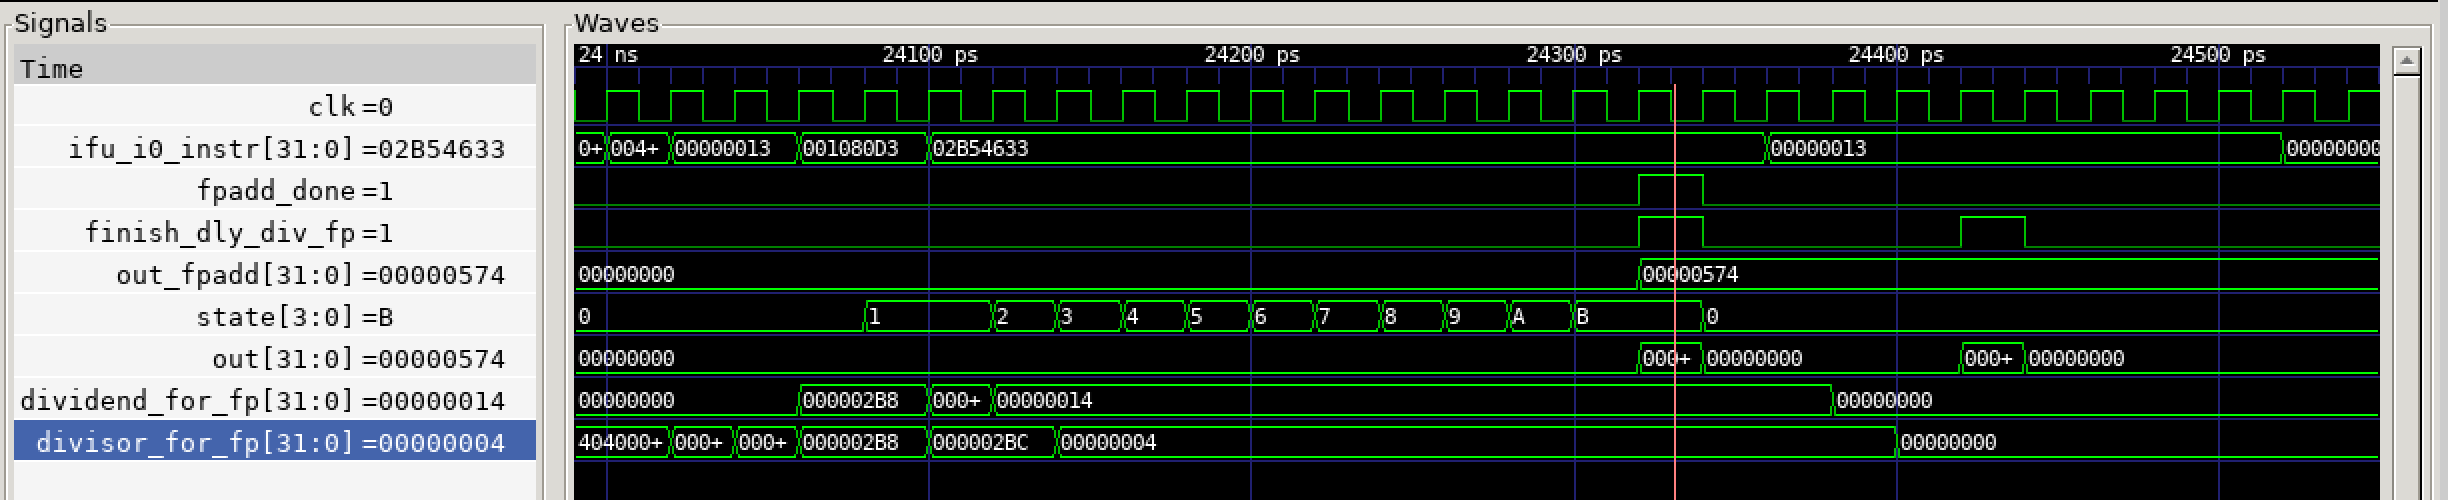
\includegraphics[width=1.0\textwidth]{pp5.png}
    \caption{错误的浮点寄存器初始化波形2}
    \label{fig:reg_init_error_input}
\end{figure}

\begin{figure}[H]
    \centering
    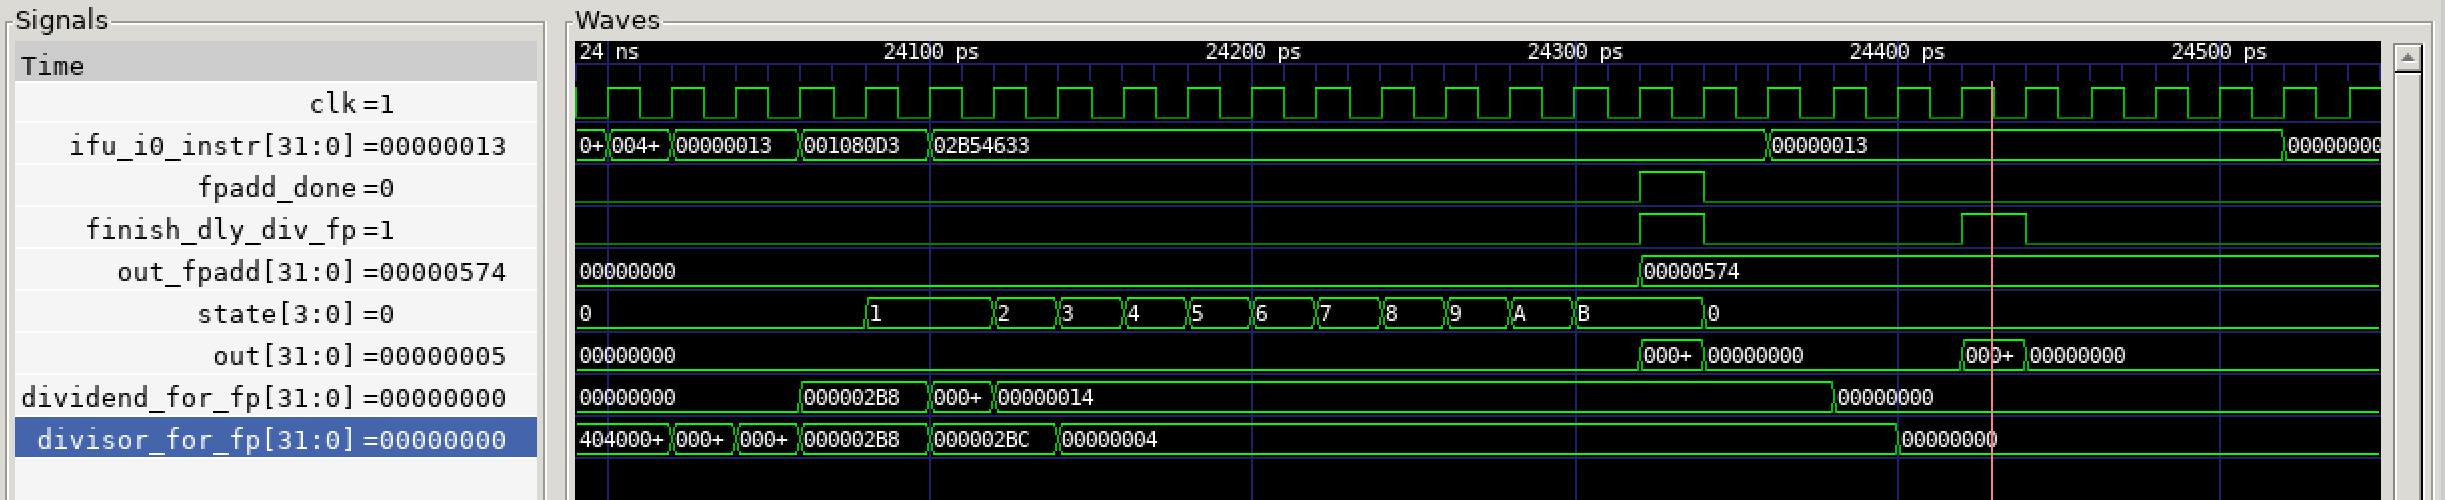
\includegraphics[width=1.0\textwidth]{pp6.png}
    \caption{错误的浮点寄存器初始化波形3}
    \label{fig:reg_init_error_output}
\end{figure}

\textbf{观察到的异常现象}（图\ref{fig:reg_init_error_state}、图\ref{fig:reg_init_error_input} 和 图\ref{fig:reg_init_error_output}）：
\begin{itemize}[itemsep=0pt, parsep=3pt]
    \item \textbf{输入数据异常}：
    \begin{itemize}[itemsep=0pt, parsep=3pt]
        \item 被加数 \texttt{dividend\_for\_fp[31:0] = 0x000002BC}（不是预期的浮点数格式）
        \item 加数 \texttt{divisor\_for\_fp[31:0] = 0x000002BC}（两个操作数异常相同）
        \item 与预期的 2.0 (0x40000000) 和 3.0 (0x40400000) 完全不符
    \end{itemize}
    
    \item \textbf{输出结果错误}：
    \begin{itemize}[itemsep=0pt, parsep=3pt]
        \item \texttt{out\_fpadd[31:0] = 0x00000574}（十进制1396）
        \item 预期应为 5.0 (0x40A00000)，结果完全错误
        \item 数值分析：\texttt{0x2BC = 700}，$700 + 700 \approx 0x574$，说明加法器在计算垃圾数据
    \end{itemize}
    
    \item \textbf{状态机仍正常执行}：
    \begin{itemize}[itemsep=0pt, parsep=3pt]
        \item \texttt{state[3:0]} 正常完成 0→1→2→...→B 转换
        \item 说明问题不在控制逻辑，而在数据来源
    \end{itemize}
\end{itemize}

\subsubsection{问题分析}

\textbf{根本原因}：\textbf{猜测是使用了未初始化的浮点寄存器}

\begin{enumerate}[itemsep=0pt, parsep=3pt]
    \item \textbf{指令解码错误}：
    \begin{lstlisting}[language=Python]
# .word 0x001080d3 实际解码为：
fadd.s f1, f1, f0
# 使用的是浮点寄存器 f0 和 f1，而非整数寄存器
    \end{lstlisting}
    
    \item \textbf{寄存器映射混淆}：
    \begin{itemize}[itemsep=0pt, parsep=3pt]
        \item \texttt{li t0, 0x40000000} 只初始化了\textbf{整数}寄存器 x5
        \item \texttt{li t1, 0x40400000} 只初始化了\textbf{整数}寄存器 x6
        \item \textbf{浮点}寄存器 f0 和 f1 从未被初始化
        \item f0、f1 包含随机值或上次执行的残留数据（0x2BC）
    \end{itemize}
    
    \item \textbf{RISC-V寄存器文件结构}：
    \begin{itemize}[itemsep=0pt, parsep=3pt]
        \item 整数寄存器（x0-x31）和浮点寄存器（f0-f31）是\textbf{独立的}物理寄存器堆
        \item 给 x5 赋值不会影响 f5
        \item 给 x6 赋值不会影响 f6
        \item \textbf{例外}：VeeR-EL2中 x28-x31 与 f28-f31 \textbf{共享物理存储}（ABI优化）
    \end{itemize}
\end{enumerate}

\subsubsection{解决方案}

\textbf{方法：利用VeeR-EL2的寄存器共享特性}

在VeeR-EL2实现中，x28-x31（t3-t6）与 f28-f31 共享同一物理寄存器，因此可以通过初始化整数寄存器来同时初始化浮点寄存器：

\begin{lstlisting}[language={[x86masm]Assembler}]
main:
    li t3, 0x40800000   # x28/f28 = 4.0（同时初始化两个寄存器文件）
    li t4, 0x40000000   # x29/f29 = 2.0
    li a3, 20
    li a4, 4

CRITICAL_TEST:
    INSERT_NOPS_4
    .word 0x01ce8f53    # fadd.s f30, f29, f28（使用共享寄存器）
    div a5, a3, a4
    INSERT_NOPS_20
\end{lstlisting}
这也就是后续测试程序 \texttt{fp\_conflict.S} 中所采用的初始化方法。

\clearpage
\section{实验总结与实验心得}

\subsection{实验完成情况}

根据Project1评分标准，本次实验完成情况如下：

\begin{enumerate}[itemsep=5pt, parsep=3pt]
    \item \textbf{基础任务（100分）}：✓ 完成
    \begin{itemize}[itemsep=0pt, parsep=3pt]
        \item 成功集成浮点加法器fp\_adder模块到VeeR-EL2处理器
        \item 完成译码级、执行级、顶层的信号修改和连接
        \item 实现自定义浮点加指令fadd.s的软硬件支持
        \item 波形分析显示状态机正常运行，计算结果正确，握手协议工作正常
    \end{itemize}
    
    \item \textbf{自定义集成方式（25分）}：✓ 完成
    \begin{itemize}[itemsep=0pt, parsep=3pt]
        \item 实现了基于FSM的握手协议集成方案
        \item 通过锁存方案和状态机方案的对比，深入理解了握手协议和数据同步问题
        \item 采用6状态FSM（IDLE→LATCH\_DATA→SEND\_A→SEND\_B→COMPUTING→COMPLETE）确保时序正确性
    \end{itemize}
    
    \item \textbf{浮点乘除法扩展（每项50分）}：✓ 完成
    \begin{itemize}[itemsep=0pt, parsep=3pt]
        \item 成功集成fp\_multiplier和fp\_divider模块（来自https://github.com/dawsonjon/fpu）
        \item 实现fmul.s和fdiv.s指令的完整软硬件支持
        \item 为每个浮点操作创建独立的FSM实例，实现4路操作选择（整数除法+浮点加/乘/除）
        \item 编写专用测试文件fp\_mul.S和fp\_div.S，并通过波形验证计算结果正确
    \end{itemize}
    
    \item \textbf{多测试文件验证（10分）}：✓ 完成
    \begin{itemize}[itemsep=0pt, parsep=3pt]
        \item 编写基础测试文件 \texttt{fp\_add.S}、\texttt{fp\_mul.S}、\texttt{fp\_div.S}（验证各浮点操作）
        \item 编写冲突测试文件 \texttt{fp\_conflict.S}（零延迟背靠背测试）
        \item 使用GTKWave深入分析波形，创建operation-specific TCL配置文件
        \item 通过IEEE 754标准验证浮点运算结果的正确性
    \end{itemize}
\end{enumerate}

\textbf{加分项总计}：25分（自定义集成）+ 100分（乘除法）+ 10分（多测试文件）= 135分

\textbf{预计总分}：100分（基础）+ 135分（加分）= 235分

\subsection{实验总结}

本次实验让我掌握了以下能力：
\begin{enumerate}[itemsep=3pt, parsep=3pt]
    \item \textbf{硬件设计能力}：深入理解了VeeR-EL2四级流水线架构，掌握了多模块并行集成技术，学会了FSM状态机设计和握手协议实现
    \item \textbf{SystemVerilog 编程}：熟练使用结构体封装信号，掌握独热码编码和位掩码多路选择，深入理解组合逻辑与时序逻辑的区别，学会了参数化模块设计
    \item \textbf{问题分析能力}：通过OR运算数据污染、握手时序错误、寄存器初始化等问题的解决，学会了系统性调试方法和边界条件测试；通过对比锁存方案和FSM方案，理解了不同设计方案的优劣
    \item \textbf{仿真调试技能}：熟练使用GTKWave进行波形分析，编写Makefile和TCL脚本实现自动化测试，掌握了IEEE 754浮点数标准及其验证方法
    \item \textbf{扩展能力}：成功从单一浮点加法扩展到加/乘/除三种运算，实现了可复用的FSM框架，为后续功能扩展打下基础
\end{enumerate}

\subsection{实验心得}

本次实验是一次从理论到实践的完整旅程。在集成浮点运算单元的过程中，我深刻
体会到硬件设计的严谨性——每一个信号的时序、每一次数据的传递都必须精确控制。
从最初OR延迟链方案的失败，到锁存方案的部分成功，再到最终采用FSM状态机实现
规范的握手协议，这个迭代优化的过程让我明白：看似合理的设计在特定场景下可能失
效，只有通过全面的测试和细致的波形分析才能发现问题本质。

在扩展乘除法功能时，我体会到了模块化设计的重要性。通过将握手协议封装为独
立的FSM，可以轻松复用到不同的浮点运算单元，这种可扩展性是优秀硬件设计的标志。
同时，在调试除法器的50次迭代过程中，我学会了区分正常的算法特性和真正的错误，
这需要对底层算法有深入理解。

更重要的是，我学会了如何在遇到问题时系统性地分析、假设、验证，这种工程思
维将使我终身受益。从单精度浮点数的IEEE 754编码验证，到多操作类型的并行集成，
每一步都加深了我对计算机组成的理解。通过这次实验，我不仅完成了三个浮点运算单
元的集成，更建立了对硬件设计方法论的深层认识，这是课堂学习无法替代的宝贵经验。

\end{document}